\documentclass[12pt,letterpaper,twoside]{report}
\usepackage{appendix}
%\usepackage[maxbibnames=99]{biblatex}
\usepackage{graphicx}
\usepackage{amsmath}
\usepackage{mathtools}
\usepackage{setspace}
\usepackage{pdfpages}
\usepackage{adjustbox}
\usepackage[byname]{smartref}
\usepackage{booktabs,tabularx}	% nicer tables
\usepackage{soul,color}
\usepackage{hyperref}			%comment out for hardcopy
\hypersetup{linkcolor=black, citecolor=black, colorlinks=false}  % Colours hyperlinks in blue, but this can be distracting if there are many links.
\usepackage{apacite}			%THIS HAS TO GO AFTER HYPERREF 
\usepackage{txfonts}
\usepackage{tocloft}
\usepackage{WUthesis}			% must follow tocloft
\pagestyle{thesis}
% Set up page layout.
\addtolength{\textheight}{1in} % Height of the main body of the text
\addtolength{\topmargin}{-.5in} % .5" margin on top of page
\setlength{\textwidth}{6.25in} % width of the body of the text
\setlength{\oddsidemargin}{0.25in} % 1.25" margin on the left for odd pages
\setlength{\evensidemargin}{0in} % 1.25"  margin on the right for even pages

\usepackage{acronym}
%%%%%%%%%%%%%%%%%%%%%%%%%%%%%%%%%%% my abbreviations
\acrodef{EEG}{electroencephalography}
\acrodef{ICA}{independent component analysis}
\acrodef{ERP}{event-related potential}
\acrodef{PCA}{principal component analysis}
\acrodef{CAE}{convolutional auto-encoder}
\acrodef{CNN}{convolutional neural network}
%\acrodef{ANN}{artificial neural network}
\acrodef{MSRE}{mean squared reconstruction error}
\acrodef{MIR}{music information retrieval}
\acrodef{BCI}{brain-computer interface}
\acrodef{SSEP}{steady state evoked potential}
\acrodef{SCE}{similarity constraint encoder}
%
\newcommand{\etal}{{et al.~}}  %% better {{\it et al}.}, and in use: \etal\ (note the trailing \ , **only when you need** the space after . )
%
%\makeatletter
%
% Make each page fill up the entire page. comment this out if you
% prefer. 
%\flushbottom
%\setcounter{tocdepth}{3} % Number the subsubsections 
%\renewcommand\baselinestretch{1.66} % default line spacing is 1
%
%\makeatother
%
%%%%%%%%%%%%%%%%%% to work on a group (not all) of chapters
%\includeonly{frontmatter,Chapters/Introduction,Chapters/Methods,Chapters/ERPResults,Chapters/DeepLearningMethods,Chapters/DeepLearningResults,Chapters/Behavioural,Chapters/Discussion}
%%%%%%%%%%%%%%%%%% to work on just one chapter at a time:
%\includeonly{Chapters/NetworkMethods}
%
\begin{document}
\renewcommand{\super}{Dr. Jessica A. Grahn} %supervisor
\renewcommand{\superj}{Dr. Adrian M. Owen} %joint supervisor, if there is one, leave blank if not (lbin)... only one of the three.
\renewcommand{\superc}{} %co-supervisor, if there is one, leave blank if not (lbin)
\renewcommand{\supera}{} %alternate supervisor, if there is one, leave blank if not (lbin)
\renewcommand{\sco}{}  %member of supervisory committee
\renewcommand{\sct}{}  %other member of supervisory committee (lbin)
\renewcommand{\examo}{Dr. Marc Joanisse}  %examining committee (up to four, if less leave blank)
\renewcommand{\examt}{Dr. Ingrid Johnsrude}
\renewcommand{\examth}{Dr. Mark Daley}
%\renewcommand{\examf}{}
\renewcommand{\department}{Department of Psychology}
\renewcommand{\degree}{Masters of Science}
\renewcommand{\firstname}{Avital}
\renewcommand{\lastname}{Sternin}
\renewcommand{\titl}{Classifying music perception and imagination using EEG}
%\renewcommand{\spinetitle}{}%only if the above is more than 60 characters
\renewcommand{\thesisformat}{Monograph} %or Integrated Article
%\renewcommand{\gyear}{\number\year}
%\newcommand{\makecoauthor}{
%Type information about coauthorship here/ }
\renewcommand{\makeacknowlege} {
%Type in acknowlegements here
}
%% This sets the page style and numbering for preliminary sections.
\begin{preliminary}
\maketitle
\addcontentsline{toc}{chapter}{Certificate of Examination}
\makecert
\newpage
%\addcontentsline{toc}{chapter}{Co-Authorship Statement}
%\coauthor{\makecoauthor}  %comment this out if none
%\newpage
%\addcontentsline{toc}{chapter}{Acknowlegements}
%\acknowlege{\makeacknowlege}	%as above
\addcontentsline{toc}{chapter}{Abstract}
\Large\begin{center}\textbf{Abstract}\end{center}\normalsize
%%  ***  Put your Abstract here.   ***
%% (150 words for M.Sc. and 350 words for Ph.D.)

This is a really silly abstract.

\vfill
\textbf{Keywords:} Time series analysis, data mining
\newpage
\tableofcontents
\newpage
\addcontentsline{toc}{chapter}{List of Figures}
\listoffigures
\newpage
\addcontentsline{toc}{chapter}{List of Tables}
\listoftables\newpage
\addcontentsline{toc}{chapter}{List of Appendices}
\listofmyappendices\newpage
%\addcontentsline{toc}{chapter}{List of Abbreviations, Symbols, and Nomenclature}
%\large List of Abbreviations, Symbols, and Nomenclature \normalsize
%\newpage
% make sure to begin the regular text on the right-hand side
% p.1 is the ODD side, wider margin on th eleft in double-sided
\cleardoublepage
\end{preliminary}
\begin{spacing}{2}
\chapter*{Introduction}
\addcontentsline{toc}{chapter}{1. Introduction}

Everybody imagines music. Imagining music can be defined as a deliberate internal recreation of the perceptual experience of listening to music \cite{schaefer_name_2011}.
Individuals can imagine themselves producing music, imagine listening to others produce music, or simply "hear" the music in their heads. 
Music imagination is used by musicians to memorize music and anyone who has ever had an "ear-worm" -- a tune stuck in their head -- has experienced imagining music. Because of its simplicity no training is required to imagine a song, and researchers have been investing the utility of music imagery for \acp{BCI}.
A \ac{BCI} is a system that allows an external device to be controlled or modified using brain activity. 
Music imagery appears to be a very promising means for driving \acp{BCI} that use \ac{EEG} -- a popular non-invasive neuroimaging technique that relies on electrodes placed on the scalp to measure the electrical activity of the brain.
For instance, Schaefer \etal\cite{schaefer_measuring_2011} argue that
\emph{``music is especially suitable to use here as (externally or internally generated) stimulus material, since it unfolds over time, and \ac{EEG} is especially precise in measuring the timing of a response.''}
For patients that have difficulties communicating behaviourally (e.g. patients with locked-in syndrome) \ac{BCI}s are a promising communication tool. 
{BCI}s that currently exist are generally binary systems that allow the user to choose between two options to answer yes/no questions. %limiting communication abilities. 
A system with a larger number of answer options would offer a more complete communication experience. 
Using music as the basis for a \ac{BCI} is a promising way to build such a system due to the large number of musical pieces that exist. 
Ideally, a music-based \ac{BCI} would allow the user to imagine a piece of music in order to convey a particular thought. 
However, the translation from music imagination will require careful processing of the EEG data. 

EEG data contain a variety of signals, elicited by sounds, that can be exploited by a \ac{BCI}. 
%However, the EEG data is full of unwanted signals (noise) and extracting the relevant information can be a challenge.
%Decoding brain wave recordings to classify different states is a relatively new field of research.
%A recent review of neuroimaging methods for \ac{MIR} that also covers techniques different from EEG is given in \cite{ismir2015kaneshiro}.
\ac{EEG} signals have been used to measure emotions induced by music perception \cite{lin_eeg_2009,cabredo_emotion_2012} and to distinguish perceived rhythmic stimuli \cite{stober2014nips}.
Further in the rhythmic domain it has been shown that oscillatory neural activity in the gamma frequency band (20-60 Hz) is sensitive to accented tones in a rhythmic sequence \cite{snyder_gamma-band_2005}.
Oscillations in the beta band (20-30 Hz) entrain to rhythmic sequences \cite{cirelli_beta_2014, merchant_beta_2015} and increase in anticipation of strong tones in a non-isochronous, rhythmic sequence \cite{iversen_top-down_2009,fujioka_beta_2009,fujioka_internalized_2012}.
The magnitude of \acp{SSEP}, which reflect neural oscillations entrained to the stimulus, changes when subjects hear rhythmic sequences for frequencies related to the metrical structure of the rhythm.
This is a sign of entrainment to beat and meter \cite{nozaradan_tagging_2011,nozaradan_selective_2012}. 
\ac{EEG} studies have further shown that perturbations of the rhythmic pattern lead to distinguishable \acp{ERP} \cite{geiser_early_2009}.
Furthermore, Vlek \etal \cite{vlek_shared_2011} showed that imagined auditory accents imposed on top of a steady metronome click can be recognized from EEG.

Recently studies have identified a close relationship between the brain areas that are active during the imagination and the perception of music \cite{halpern_fmri_2004,Kraemer2005,Herholz2008,herholz_2012}. 
Although not directly relevant to a \ac{BCI}, we can learn a lot from \ac{EEG} data collected while participants listen to melodies.
Exploring EEG data during music perception can inform how we approach music imagination data and the brain signals recorded while listening to music could serve as reference data to determine which salient elements are to be expected during imagination. 
By using perception data as a way to train our \ac{BCI} we can cut down on the amount of imagination training needed which will reduce potential user fatigue.

EEG has already successfully been used to classify perceived melodies. 
In a study by Schaefer \etal \cite{schaefer_name_2011}, 10 participants \textit{listened} to 7 short melody clips with a length between 3.26s and 4.36s.
For single-trial classification, each stimulus was presented 140 times in randomized back-to-back sequences of all stimuli.
Using a quadratically regularized linear logistic-regression classifier with 10-fold cross-validation, they were able to successfully classify the \acp{ERP} of single trials.
Within subjects, the accuracy varied between 25\% and 70\%.
Applying the same classification scheme across participants, they obtained between 35\% and 53\% accuracy.
%In a further analysis, they combined all trials from all subjects and stimuli into a grand average \ac{ERP}.
%Using singular-value decomposition, they obtained a fronto-central component that explained 23\% of the total signal variance.
%The time courses corresponding to this component showed significant differences between stimuli that were strong enough to allow cross-participant classification.
%As Hubbard concludes in his recent review of the literature on auditory imagery, \emph{``auditory imagery preserves many structural and temporal properties of auditory stimuli''} and \emph{``involves many of the same brain areas as auditory perception''} \cite{hubbard_auditory_2010}. 
%This is also underlined by Schaefer \cite[p. 142]{schaefer_measuring_2011} whose \emph{``most important conclusion is that there is a substantial amount of overlap between the two tasks} [music perception and imagination]\emph{, and that `internally' creating a perceptual experience uses functionalities of `normal' perception.''}

Brain activity during music imagination has also been detected by \ac{EEG} \cite{schaefer_shared_2013}, and encouraging preliminary results for recognizing imagined music fragments from \ac{EEG} recordings were reported in \cite{schaefer_single_2009} in which 4 out of 8 participants produced imagery that was classifiable (in a binary comparison) with an accuracy between 70\% and 90\% after 11 trials.

Although \ac{EEG} has been used to decode music imagination the accuracy levels are not robust enough for these decoding techniques to be used in a \ac{BCI}. 
This could be because the EEG processing methods may not be sensitive enough to the subtle changes that occur during music imagination. 
The sophisticated signal processing techniques used in machine learning can lend expertise to this challenge. 

Machine learning is a technique that uses algorithms that can learn from and make predictions about data.
For example, the programs used by postal services to recognize handwriting on envelopes or the speech recognition software in your cell phone are based on machine learning techniques.
One such technique is based on convolutional neural networks (\acp{CNN}).
\acp{CNN} were inspired by the powerfully complex visual system found in humans and other animals.
In the retina we have cells that are responsive to small regions of the visual field \cite{hubel_receptive_1963}. 
As information moves along the visual processing stream and into the brain single cells in higher layers receive input from multiple cells in lower layers.
At each level of this process more information is combined.
This gives cells higher up in the processing stream an increasingly global view of what information was collected by the retinal cells.
Complex visual information is processed farther along the processing stream than simple information as cells in these far layers are sent information from a larger number of retinal cells.
\acp{CNN} work in a similar way to process complex data. 
The processing units in a \ac{CNN} act like cells in the visual system.
The ``receptive field'' of each one of these units is determined by a filter.
Each filter is created based on a variety of parameters set by the researcher or determined by the network during the training process.
%In this experiment the filters used are \acp{CAE} (as described in \cite{masci_stacked_2011}).
%A \ac{CAE} is an artificial neural network that is able to extract features from data without supervision.
% feature extractor that scales well to high dimensional input.
%CAEs are a special variant of a \ac{CNN} that encode their input using convolution into a compressed internal representation. 
%This representation is then decoded using de-convolution into the original space while trying to minimize the reconstruction error. 
%This type of neural network can learn a meaningful but compressed representation of the data.
%Importantly, \acp{CAE} preserve spatial information allowing them to learn biologically plausible features.%
%Once the \ac{CAE} has extracted the important features from the training data and constructed the filters these filters can be used in a \ac{CNN}.
%These filters are very similar to the components produced in \ac{PCA} and \ac{ICA} with the difference being the parameters used to compute the components. 
%The \ac{CAE} filters aim to minimize the \ac{MSRE} rather than the orthogonality or independence criteria used in \ac{PCA} and \ac{ICA} respectively. 
Before a \ac{CNN} can be used to classify data it must learn the characteristics of the data. 
The \ac{CNN} is trained using a subset of the data and the filters are optimized to produce the best classification results. 
The optimized filters are applied to new data and the accuracy of the classification is determined. 

%SUMMARY OF WHAT WE TRIED AND THE TECHNIQUES WE USED
%Using this analysis technique we aim to be able to classify what a participant was listening to or imagining based on the signal in their EEG data alone. 
To approach this problem we first tried an ERP analysis similar to that of Schaefer \etal\cite{schaefer_name_2011} in order to determine which piece of music a participant was listening to or imagining.
When this proved unsuccessful we used a machine learning technique called deep learning to detect more subtle differences in the EEG that would be more useful in classifying stimuli. 
Using this technique we were able to classify perception of 12 music pieces with a 28.7\% accuracy (chance=8.3\%).
We were unable to accurately classify imagination of music \hl{specific values go here}.
\section*{Methods}
\addcontentsline{toc}{chapter}{Methods}
\subsection*{Participants}
Fourteen participants (3 male), aged 19-36, with normal hearing and no history of brain injury took part in this study. Eight participants had formal musical training (1- 26 years), and four of the participants played instruments regularly at the time of data collection.
\vspace{-0.5em}
\subsection*{Stimuli}
Stimuli were fragments of familiar musical pieces and were selected based on key signature (3/4 or 4/4 time) and the presence and absence of lyrics. The stimuli were kept as similar in length as possible with care taken to ensure that they all contained complete musical phrases. Stimulus details can be found in \autoref{tab:stimuli_information}.
Each musical fragment was preceded by approximately two seconds of clicks as a cue to the tempo and onset of the music. The beats began to fade out at the one second mark and stopped at the onset of the music. 
\begin{table}[t]
%\vspace{-1em}
\setlength{\tabcolsep}{2.5pt}  % use to control space between columns
\renewcommand{\arraystretch}{1}
\centering
\caption{Information about the tempo, meter and length of the stimuli used in this experiment.}
%Mean and standard deviation over individual subjects.}
\label{tab:stimuli_information}
{\footnotesize % \sffamily \fontfamily{anttlc}\selectfont
%{\small % \sffamily \fontfamily{anttlc}\selectfont
\begin{tabularx}{\columnwidth}{r l c c  c c c }
\toprule
ID		& Name							&Meter 	& Length	& Tempo 		&\#Bars	& Bar Length\\
\midrule
1		& Chim Chim Cheree (lyrics)			& 3/4		& 13.3s 			& 212 BPM 	& 16				& 0.85s	\\ % ($\ge$12 bars)\\
2		& Take Me Out to the Ballgame (lyrics)	& 3/4		& 7.7s 			& 189 BPM 	& 8				& 0.95s	\\ % ($\ge$9 bars)\\
3		& Jingle Bells (lyrics)					& 4/4		& 9.7s 			& 200 BPM 	& 8				& 1.20s	\\ % ($\ge$12 bars)\\
4		& Mary Had a Little Lamb (lyrics)		& 4/4		& 11.6s			& 160 BPM 	& 8				& 1.50s	\\ % ($\ge$12 bars)\\
11		& Chim Chim Cheree 				& 3/4		& 13.5s	 		& 212 BPM 	& 16				& 0.85s	\\ % ($\ge$12 bars)\\
12		& Take Me Out to the Ballgame			& 3/4		& 7.7s 			& 189 BPM 	& 8				& 0.95s	\\ % ($\ge$9 bars)\\
13		& Jingle Bells 						& 4/4		& 9.0s 			& 200 BPM 	& 8				& 1.20s	\\ % ($\ge$12 bars)\\
14		& Mary Had a Little Lamb				& 4/4		& 12.2s			& 160 BPM 	& 8				& 1.50s	\\ % ($\ge$12 bars)\\
21		& Emperor Waltz					& 3/4		& 8.3s 			& 178 BPM 	& 8				& 1.01s	\\ % ($\ge$12 bars)\\
22		& Hedwig's Theme (Harry Potter)		& 3/4		& 16.0s	 		& 166 BPM 	& 15				& 1.08s	\\ % ($\ge$9 bars)\\
23		& Imperial March (Star Wars Theme)		& 4/4		& 9.2s 			& 104 BPM 	& 4				& 2.30s	\\ % ($\ge$12 bars)\\
24		& Eine Kleine Nachtmusik				& 4/4		& 6.9s			& 140 BPM 	& 4				& 1.71s	\\ % ($\ge$12 bars)\\
\bottomrule
\end{tabularx}
}
%\vspace{-1em}
%\vspace{-0.8em}
\end{table}

\subsection*{Equipment and Procedure}
\subsubsection*{Behavioural Testing}
We collected information about the participants' previous music experience, their ability to imagine sounds, and information about musical sophistication using an adapted version of the widely used Goldsmith's Musical Sophistication Index (G-MSI) \cite{mullensiefen_musicality_2014} combined with an adapted clarity of auditory imagination scale \cite{willander_imagery_scale_2010}. 
We also had participants complete a beat tapping and a stimuli familiarity task. 
Participants listened to each stimulus and were asked to tap along with the music on the table top. The experimenter then rated their tapping ability on a scale from 1 (difficult to assess) to 3 (tapping done properly). 
After listening to each stimulus participants rated their familiarity with the stimuli on a scale from 1 (unfamiliar) to 3 (very familiar).
To participate in the \ac{EEG} portion of the study, the participants had to receive a score of at least 90\% on our beat tapping task. Participants received scores from 75\%--100\% with an average score of 96\%.
Furthermore, they needed to receive a score of at least 80\% on our stimuli familiarity task. 
Participants received scores from 71\%--100\% with an average score 87\%.
These requirements resulted in rejecting 4 participants.
This left 10 participants (3 male), aged 19--36, with normal hearing and no history of brain injury. 
These 10 participants had an average tapping score of 98\% and an average familiarity score of 92\%.
Eight participants had formal musical training (1--10 years), and four of those participants played instruments regularly at the time of data collection.

\subsubsection*{EEG recording}
For the EEG portion of the study, the 10 participants were seated in an audiometric room (Eckel model CL-13) and connected to a BioSemi Active-Two system recording 64+2 EEG channels at 512 Hz as shown in \autoref{fig:eegsetup}.
\begin{figure}
  \begin{center}
    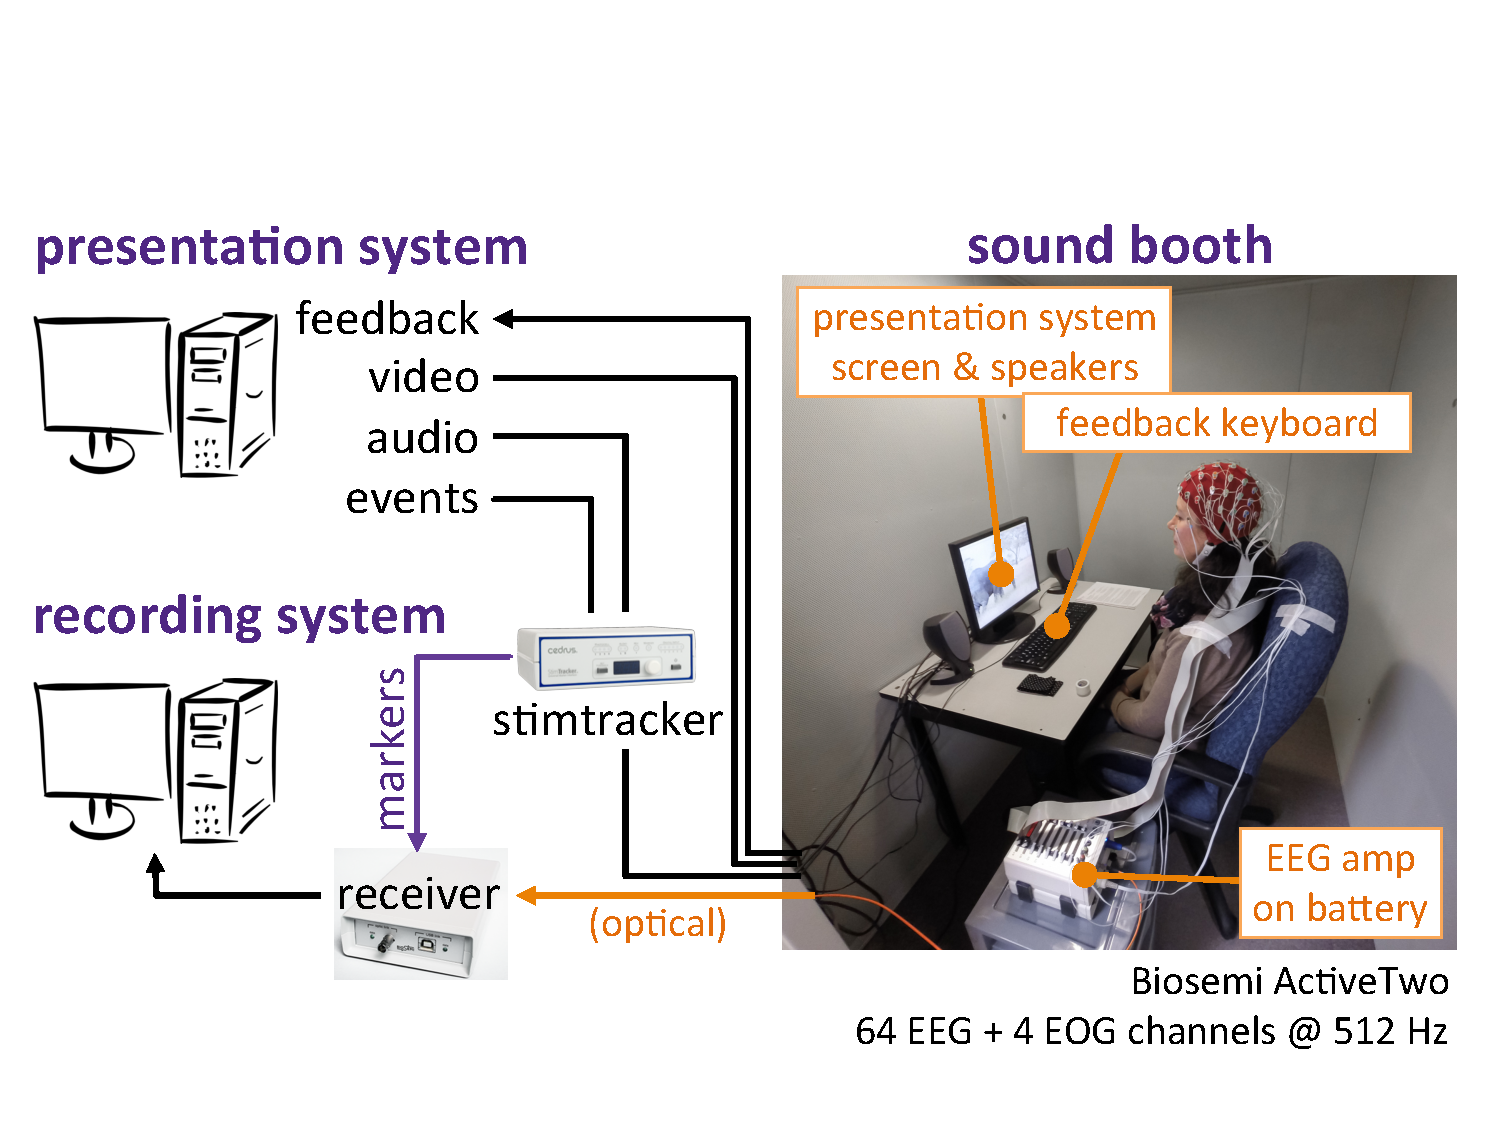
\includegraphics[width=\columnwidth,keepaspectratio=true]{Figures/EEG-setup.pdf}
%   \\\vspace{-0.8em}
    \caption{%
Setup for the EEG experiment.
The presentation and recording systems were placed outside to reduce the impact of electrical line noise that could be picked up by the EEG amplifier.
}
    \label{fig:eegsetup}
  \end{center}
% \vspace{-2em}
\end{figure}
Horizontal and vertical EOG channels were used to record eye movements. 
We also recorded the left and right mastoid channel as EEG reference signals. 
Due to an oversight, the mastoid data was not collected for the first 5 subjects.
The presented audio %and the recorded EEG were 
was routed through a Cedrus StimTracker connected to the EEG receiver, which allowed a high-precision synchronization ($<$0.05 ms) of the stimulus onsets with the \ac{EEG} data.
The experiment was programmed and presented using PsychToolbox run in Matlab 2014a. 
A computer monitor displayed the instructions and fixation cross for the participants to focus on during the trials to reduce eye movements.
The stimuli and cue clicks were played through speakers at a comfortable volume that was kept constant across participants. Headphones were not used because pilot participants reported headphones caused them to hear their heartbeat which interfered with the imagination portion of the experiment. 
After the experiment, we asked participants the method they used to imagine music. 
The participants were split evenly between imagining themselves producing the music (singing or humming) and simply ``hearing the music in [their] head.'' 

The EEG experiment was divided into 2 parts with 5 blocks each as illustrated in \autoref{fig:experiment_outline}.
% Note: 	the figure won't be place exactly here (this would require [h]. [t] stands for "top")
%			This just makes sure, it comes after the 1st reference
\begin{figure*}
  \begin{center}
    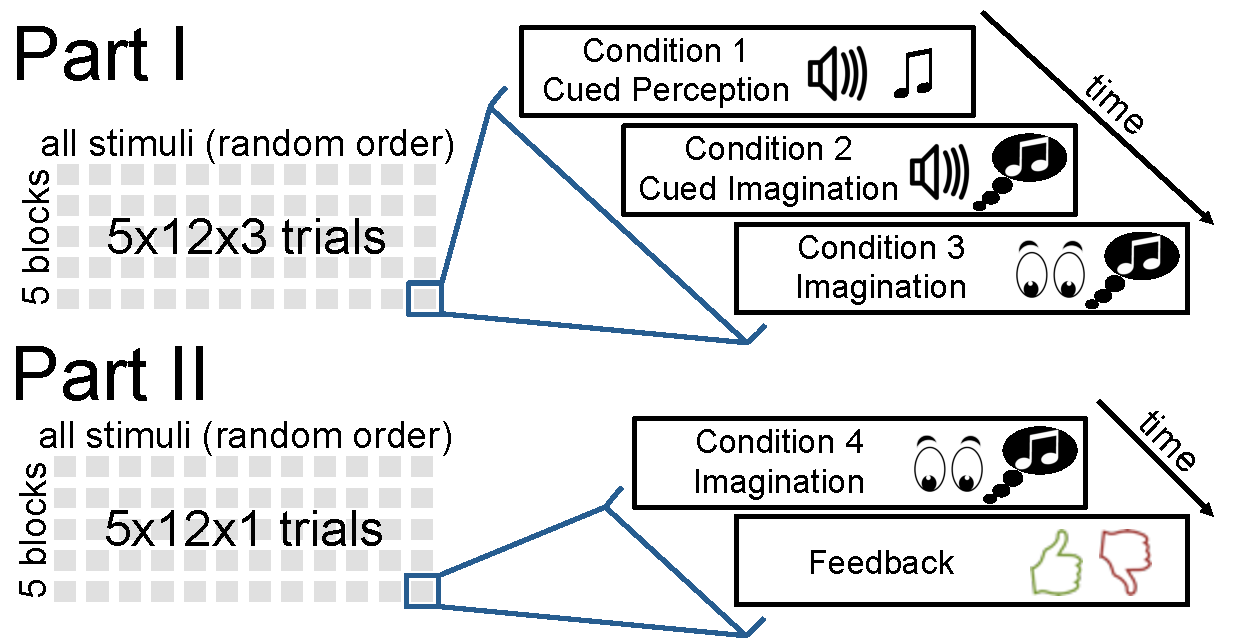
\includegraphics[width=0.8\textwidth,keepaspectratio=true]{Figures/study_design_small.pdf}
%   \\\vspace{-0.8em}
    \caption{%
Illustration of the design for the EEG portion of the study.
}
    \label{fig:experiment_outline}
  \end{center}
%  \vspace{-2em}
\end{figure*}

A single block comprised of all 12 stimuli in randomized order.
Between blocks, participants could take breaks at their own pace.
We recorded EEG in 4 conditions:
\begin{enumerate}
\item
Stimulus perception preceded by cue clicks
\item
Stimulus imagination preceded by cue clicks
\item
Stimulus imagination without cue clicks
\item
Stimulus imagination without cue clicks, with feedback
\end{enumerate}
The goal was to use the cue to align trials of the same stimulus collected under conditions 1 and 2. Lining up the trials allows us to directly compare the perception and imagination of music and to identify overlapping features in the data. 
Conditions 3 and 4 simulate a more realistic query scenario during which the system does not have prior information about the tempo and meter of the imagined stimulus.
These two conditions were identical except for the trial context.
While the condition 1--3 trials were recorded directly back-to-back within the first part of the experiment, 
all condition 4 trials were recorded separately in the second part, without any cue clicks or tempo priming by prior presentation of the stimulus.
After each condition 4 trial, participants provided feedback by pressing one of two buttons indicating on whether or not they felt they had imagined the stimulus correctly.
In total, 240 trials (12 stimuli x 4 conditions x 5 blocks) were recorded per subject.
%
The event markers recorded in the raw EEG comprise:
\begin{itemize}
\item
	Trial labels (as a concatenation of stimulus ID and condition) at the beginning of each trial
\item
	Exact audio onsets for the first cue click of each trial in conditions 1 and 2 (detected by the Stimtracker)
\item
	Subject feedback for the condition 4 trials (separate event IDs for positive and negative feedback)
\end{itemize}	


%We are interested in estimating the tempo of the music stimuli from the EEG signal. 
%Our analyses here focus on the data gathered during the three conditions in the first block of the experiment. Participants reported that they were not confident in their performance on the trials collected from the second block of the experiment, therefore the data were excluded from analyses and will require further attention. %
%Basic EEG preprocessing techniques were used to remove artifacts and a dynamic beat tracker was used to estimate average tempo. 
%Autocorrelation curves were computed to investigate the periodicity seen in the average EEG waveforms and the peaks from these curves were found to be proportional to stimulus bar length. 
%To deal with the tempo variance that inevitably occurred during the music imagination trials, we used a sliding window to aggregate over all channels and computed a more accurate tempo value.

\subsection*{Preprocessing}
The raw EEG and EOG data were processed using the MNE-Python toolbox. 
For recordings with additional mastoid channels, the EEG data was re-referenced by subtracting the mean mastoid signal \cite{teplan_fundamentals_2002}.
We then removed and interpolated bad EEG channels identified by manual visual inspection.
For interpolation, the spherical splines method described in \cite{perrin_spherical_1989} was applied.
The data were then filtered with an fft-bandpass, keeping a frequency range between 0.5 and 30 Hz.
This also removed any slow signal drift in the EEG.
Afterwards, we down-sampled to a sampling rate of 64 Hz.
To remove artifacts caused by eye blinks, we computed independent components using extended Infomax \ac{ICA} \cite{lee_independent_1999} and semi-automatically removed components that had a high correlation with the EOG channels.
Finally, the 64 EEG channels were reconstructed from the remaining independent components without reducing dimensionality.
%\section*{Tempo Results}
\addcontentsline{toc}{chapter}{Tempo Results}
\subsection*{Participants}
Five participants (1 male), aged 19-36, with normal hearing and no history of brain injury took part in this study. Four participants had formal musical training (1- 26 years), but none of the participants played instruments regularly at the time of data collection.

\subsection*{Analysis of Beat and Bar-Aligned ERPs}

We analyzed the music stimuli with the dynamic beat tracker \cite{Ellis2007beat} provided by the \emph{librosa} library.\footnote{%
\url{https://github.com/bmcfee/librosa}}
This way, we obtained an estimation of the average tempo as well as annotations for all beats. % (TOTAL NUMBER).
The quality of these automatic annotations was verified through sonification.

Given the beat annotations of the stimuli and assuming that our participants would imagine the stimuli at a similar tempo, 
%we extracted epochs 
%aligned to each beat (excluding cue clicks) and to each bar.
%This resulted in a total of 4x1835 per participant beat-aligned epochs starting XXXms before and ending XXXms after each beat annotation. 
%TODO: timing
%The grand averages are shown in \autoref{fig:beat-aligned grand average} separated by condition.
%TODO: Figure. What can we see? N100? More blurring expected for imagination conditions.
%Maybe, this could be used to develop a beat-detection algorithm -- but we leave this possibility for future work.
%For the bar-aligned ERPs, 
we computed bar-aligned ERPs using non-overlapping epochs from 100ms before to 2.4s after a downbeat annotation.
This length was required to capture slightly more than a single bar for the slowest stimulus -- number 23 with a bar length of more than 2.3s.
As expected, the resulting averaged ERPs differ considerably between participants, stimuli, and conditions.
However, we often observed a periodicity in the averaged signal proportional to the bar length.
%
\autoref{fig:non-overlap_bar-aligned-ERPs} shows example ERPs 
%resulting from averaging non-overlapping epochs from 100ms before to 2.4s after a downbeat annotation.
for a specific participant and stimulus where this is clearly visible in all conditions.

\begin{figure}[t]
  \begin{center}
    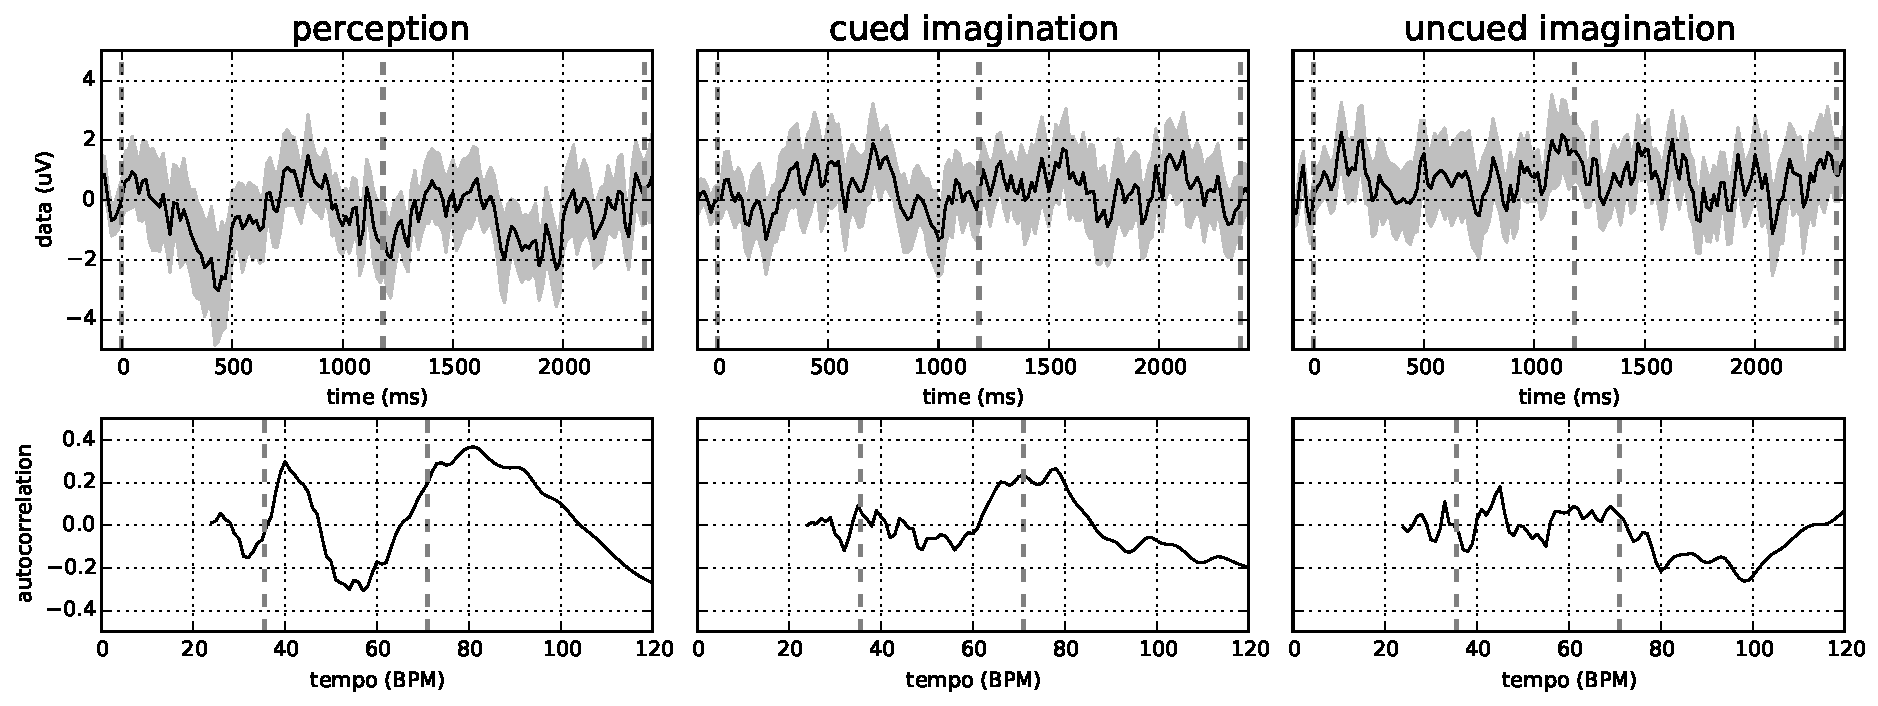
\includegraphics[width=\textwidth,keepaspectratio=true]{Figures/non-overlap_bar-aligned-ERPs.pdf}
%   \\\vspace{-0.8em}
    \caption{%
%\textit{beats are roughly evenly spaced - these peaks are not. looks like onset detection not beat detection. Would cause over-estimation of tempo (makes it seem faster than it is - Jessica)}
Top: Mean and standard deviation over all 64 EEG channels of the bar-aligned ERPs
(without epochs overlap)
for ``Chim Chim Cheree (lyrics)'' in conditions 1--3 for participant P01.
Each ERP was averaged over 25 epochs (5 from each trial).
Bottom: Corresponding autocorrelation scores in the relevant tempo range.
Dashed lines indicate downbeats (top) and the approximate bar tempo of the stimulus plus its lower tempo harmonic (bottom).
%NOTE: downbeat times are based on audio beat detection in stimulus!
}
    \label{fig:non-overlap_bar-aligned-ERPs}
  \end{center}
%  \vspace{-3em}
\end{figure}

In order to analyze this periodicity, we computed the autocorrelation curves by comparing each signal with itself at a range of time lags.
To this end, we aggregated all 64 EEG channels into a mean signal.
We further chose time lags corresponding to the bar tempo range of our stimuli.
The lower end of 24 BPM was determined by our choice of the epoch length. 
Using longer epochs would allow us to extend the tempo range to slower tempi, but this would be at the expense of fewer epochs available for averaging.
%\hl{the following sentence is unclear - slower tempo/bigger epochs} With longer epochs, the tempo range could be extended further towards zero at the expense of fewer epochs available for averaging.

In general, more distinct peaks in the autocorrelation were observed in the perception condition.
For the two imagination conditions, peaks were more blurred as can also be seen in \autoref{fig:non-overlap_bar-aligned-ERPs}.
This is most likely caused by the lack of a time locking mechanism, which allows the tempo to vary.
This hypothesis is also backed by the observation that artificially jittering the bar onsets results in a decrease in autocorrelation.

Most notably, we ensured that the bar-aligned epochs did not overlap by rejecting some of the epochs.
If they overlap, a single data segment can contribute to multiple epochs at different time points.
This can induce misleading autocorrelation peaks that are not supported by the raw data.


\subsection*{Analyzing Single Trials}

With the interesting observations reported in the preceding section, the question arises whether the tempo could similarly be estimated through autocorrelation from single trials. 
Single trial tempo estimation is important for our BCI in order to reduce patient fatigue during use.
Here, we face several challenges. 
First, there are too few bar-aligned epochs in a single trial to use ERPs.
Second, we neither know the tempo of the stimulus nor do we have beat annotations available.
Therefore, there are no reference points for extracting bar-aligned epochs.
Moreover, we wanted to address the problem of possible tempo variance in the imagination conditions.

\autoref{fig:sliding-window-analysis} illustrates our proposed solution to this problem.
We move a 2.5-second sliding window over the mean EEG signal aggregated over all channels.
At each position with a hop size of 5 samples at 64Hz, we compute the autocorrelation curve.
The curves for the individual window segments are stacked into a 2-dimensional matrix with the first dimension corresponding to the window offset in the trial signal and the second dimension corresponding to the possible tempo values.
Hence, each matrix value holds the score for a certain tempo at one specific point in the trial.
The scores in the matrix are finally aggregated deriving an estimated tempo value for the trial.
\autoref{fig:sliding-window-analysis} shows how the mean and maximum values are aggregated over all matrix rows.

\begin{figure}[t]
  \begin{center}
    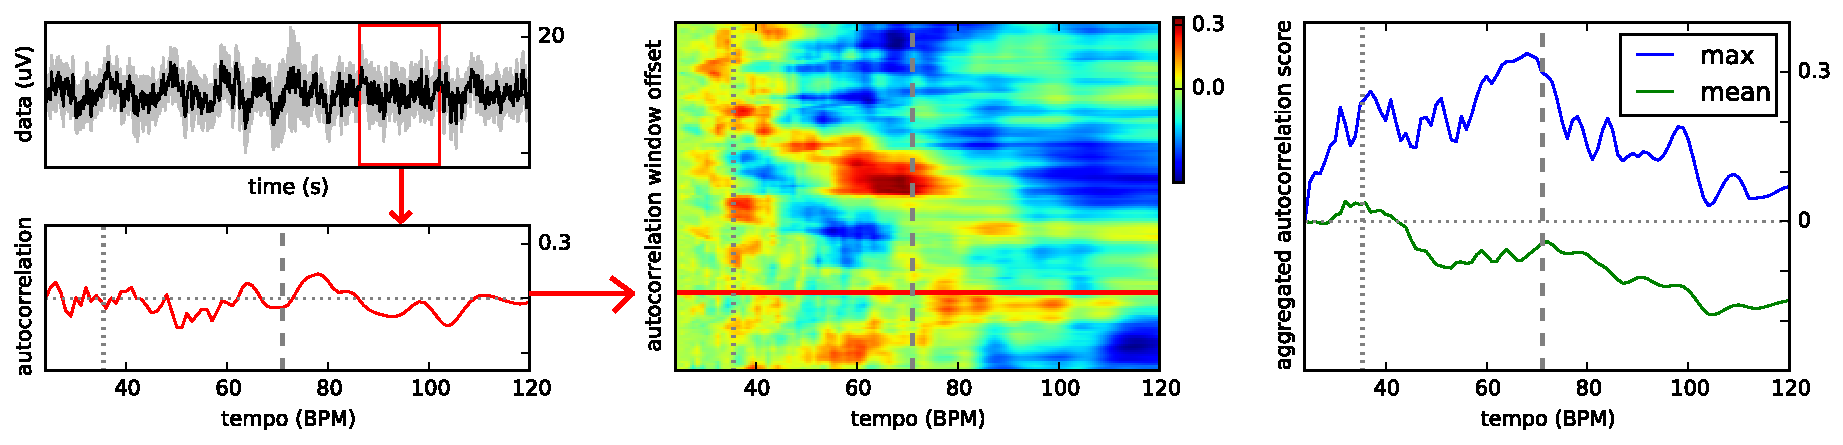
\includegraphics[width=\textwidth,keepaspectratio=true]{Figures/sliding-window-analysis_arrow.pdf}
%    \\\vspace{-0.8em}
    \caption{%
Schema of the proposed tempo estimation technique.
All plots refer to the first of the five trials contributing to the imagination ERP of ``Chim Chim Cheree (lyrics)'' in  \autoref{fig:non-overlap_bar-aligned-ERPs}, middle.
Left top: EEG waveform (mean of all 64 channels) for the whole trial with the red box indicating the sliding window of 2.5 seconds.
Left bottom: Autocorrelation curve for this specific segment of the trial.
Middle: Vertically stacked autocorrelation curves for the whole trial with the red horizontal line indicating the position of the sliding window shown on the left.
Right: Aggregated autocorrelation scores (mean and max) for the whole trial.
Dashed vertical lines indicate the stimulus bar tempo.
Dotted vertical lines refer to half the bar tempo.
    }
    \label{fig:sliding-window-analysis}
  \end{center}
%  \vspace{-2em}
\end{figure}

Ideally, the score for the actual tempo should be stable throughout the whole trial.
However, we observed substantial fluctuation within many trials.
While the mean and maximum over all matrix rows often produce significant peaks in the aggregated autocorrelation curve, the following heuristic has led to slightly more stable results:
\begin{enumerate}
\item
        In each row, find the pair of tempo values with the maximal combined score.
\item
        Select the median of all selected pairs.
\item
        From this pair, return the tempo value with the higher mean value over
all rows.
\end{enumerate}

For the evaluation of our heuristic, we computed the mean absolute error of the estimated tempo and the actual tempo.
We also considered the tempo harmonic below and above the correct value, i.e. half or twice the tempo, as a correct result.
The prediction error, averaged across all stimuli, varied considerably between participants ranging from 7.07, 7.15, and 8.11 in the three conditions for participant P14 up to 9.81, 10.04, and 12.58 for P12.
\autoref{fig:tempo-error-per-stim-cond} summarizes the errors for each stimulus over all trials of all participants.
The figure clearly shows a trend that tempo is easier to predict for some stimuli, such as ``Chim Chim Cheree'' (ID 1 and 11) and ``Mary had a little lamb'' (ID 4 and 14), than for others.
The slowest stimulus, the ``Imperial March'' (ID 23) has the highest variation of prediction accuracy.
Although it is too early to draw definitive conclusions, the data also suggest that single-trial tempo estimation does not depend on the condition (perception or imagination) but rather relies on the tempo of a stimulus.

\begin{figure}
  \begin{center}

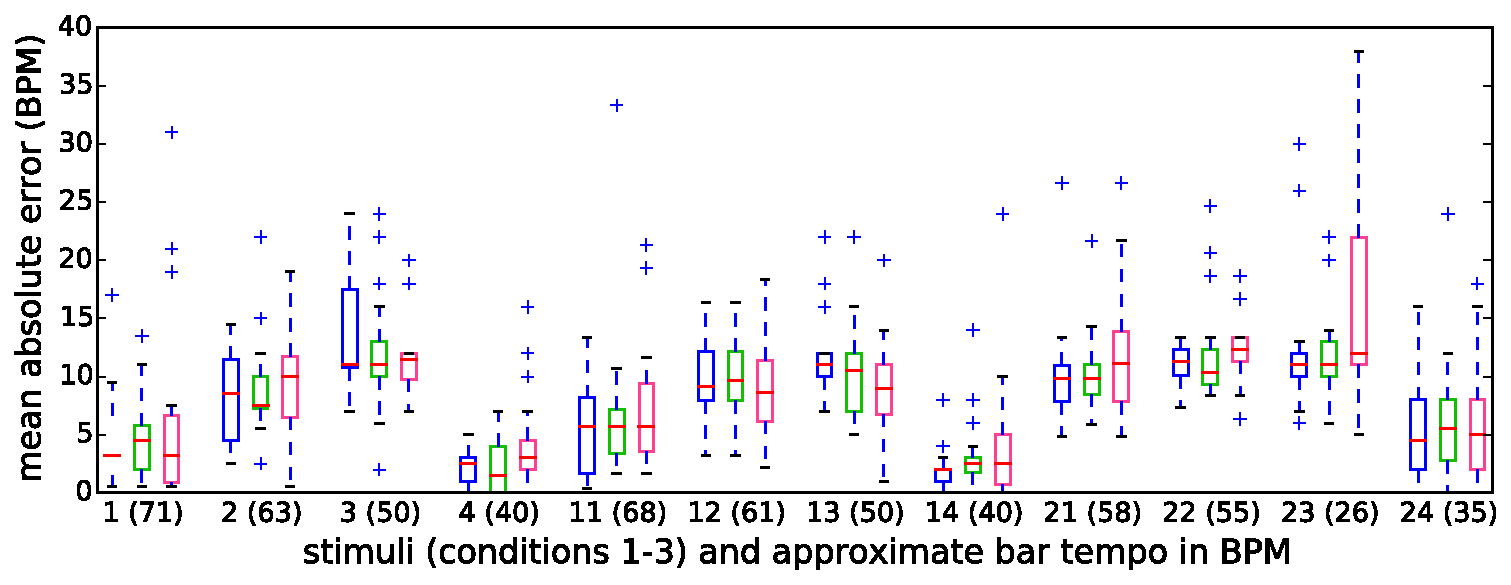
\includegraphics[width=\textwidth,keepaspectratio=true]{Figures/tempo-error-per-stim-cond-all_colour.pdf}
%  \\\vspace{-0.8em}
    \caption{Aggregated errors of single trial tempo prediction over all 5 participants. The true tempo is indicated in brackets with the mean absolute error for each stimulus indicated with a red bar. Each box contains 50\% of the error values for perception (blue), cued imagination (green) and uncued imagination (magenta). The whiskers contain an additional 25\% of the error values. Each cross indicates an outlier. }
    \label{fig:tempo-error-per-stim-cond}
  \end{center}
%  \vspace{-2em}
\end{figure}

\chapter*{ERP Analysis}
\addcontentsline{toc}{chapter}{3. ERP Analysis}
%As proposed in \cite{schaefer_name_2011}, we computed grand average \acp{ERP} by aggregating over all trials (excluding the cue clicks) of the same stimulus from all subjects except P05 (due to the movement artifacts).
Our first analysis of the data followed a strategy similar to the one used in \cite{schaefer_name_2011}.
Schaefer \etal \cite{schaefer_name_2011} used very short stimuli (3.26s) allowing each stimulus to be repeated many times during during the experiment. 
This allowed them to average across hundreds of short trials. 
They then concatenated the grand average ERPs and applied a \ac{PCA}, which resulted in clearly defined spatial features. 
The differences in the time courses of these spatial features allowed for classification of their stimuli. 
We tried to replicate these results, but we had fewer repetitions of our stimuli. 
Therefore, to preserve as much data as possible we used the full length of the trials as opposed to the first 3.26 seconds. 
We computed grand average \acp{ERP}s by aggregating over the full length of all trials (excluding the cue) of the same stimulus from all subjects. 
We then concatenated the grand average \acp{ERP} and applied a \ac{PCA}. 
This resulted in principle components with poorly defined spatial components \autoref{fig:components} (A and B).

In order to preserve even more of the data and we took an alternative approach. 
All of the raw trials were concatenated to create a single, long trial that contained all of the raw EEG information.
We ran a \ac{PCA} on the concatenated raw trials without first calculating an average across trials. 
This produced clearly defined spatial components \autoref{fig:components} (C and D). 
Except for their (arbitrary) polarity the components are very similar across the two conditions, which replicates the results found in \cite{schaefer_name_2011}.

\begin{figure}[t] 
  \begin{center}
%    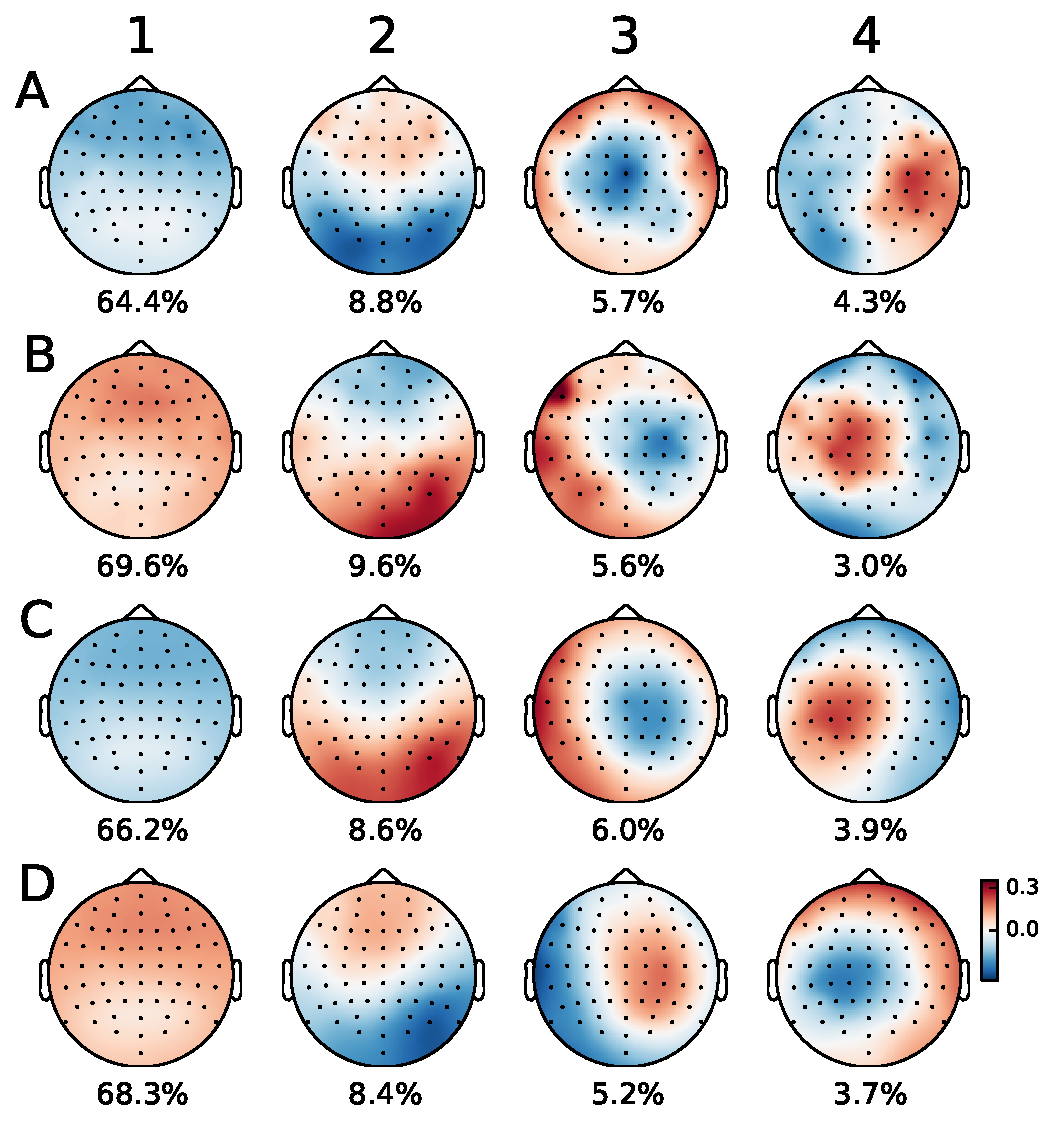
\includegraphics[width=0.8\textwidth,keepaspectratio=true]{Figures/principle_components.pdf}
    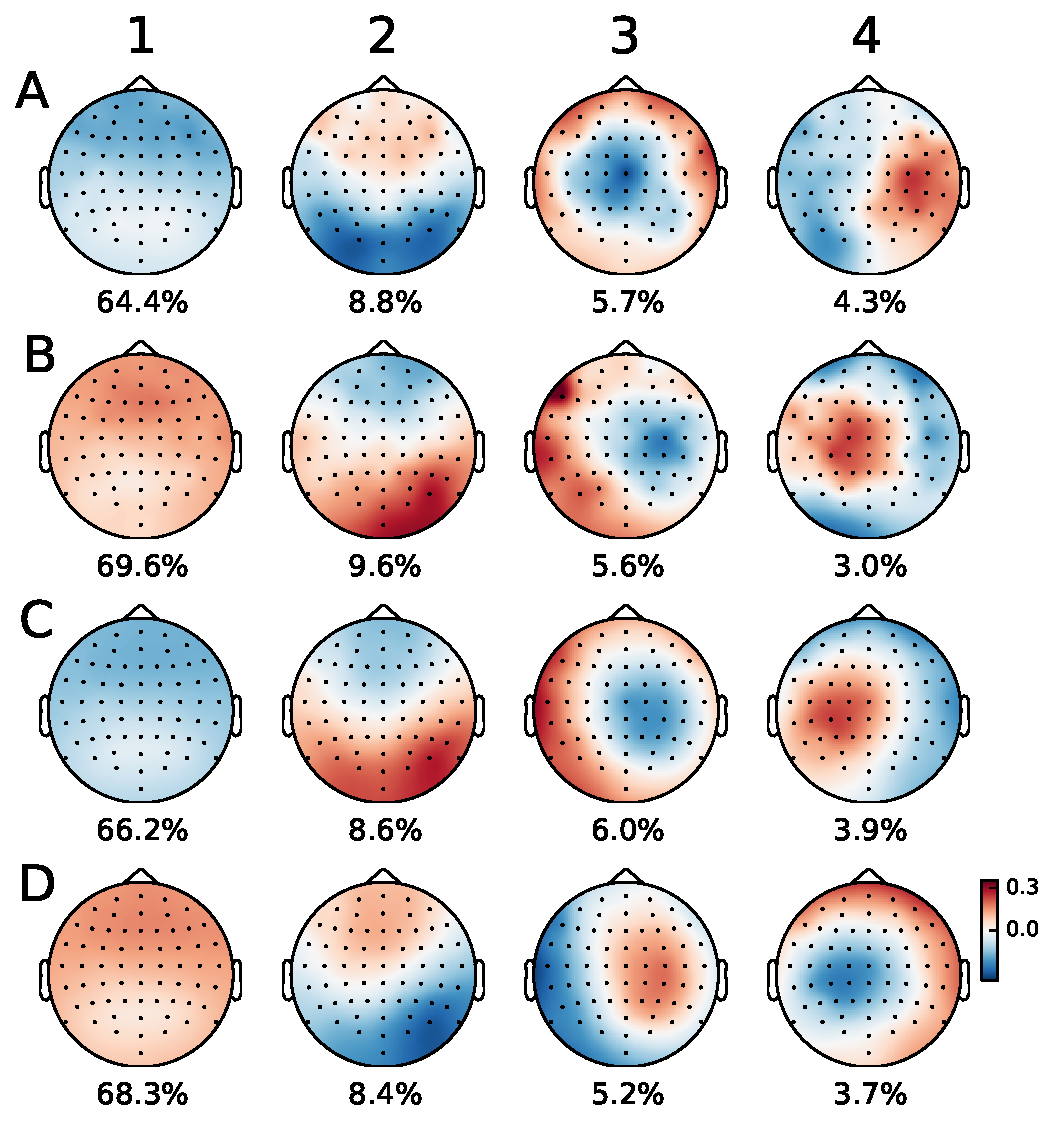
\includegraphics[scale=0.5]{Figures/principle_components.pdf}
%   \\\vspace{-0.8em}
    \caption{%
Topographic visualization of the top 4 principle components with percentage of the explained signal variance. %.\newline
Channel positions in the 64-channel EEG layout are shown as dots.
Colors are interpolated based on the channel weights.
%\hl{Polarity has no specific semantic.}
The PCA was computed on
\textbf{A}: the grand average \acp{ERP} of all perception trials,
\textbf{B}: the grand average \acp{ERP} of all cued imagination trials,
\textbf{C}: the concatenated perception trials,
\textbf{D}: the concatenated cued imagination trials.
}
    \label{fig:components}
  \end{center}
% \vspace{-2em}
\end{figure}

\subsection*{Component Waveform Correlations}
In order to investigate how similar the activation of these components is across conditions and stimuli we took the time course of component three over the first three seconds of each stimulus during perception and imagination and performed a correlation.
We used component three as it accounts for the most variance while being similar to a typical auditory component.
The highest correlations produced by this component is r=0.40 (p$<$0.001) for ``Eine Klein Nachtmusic'' (\autoref{fig:nachtmusic}) and r=0.30 (p$<$0.001) for ``The Emperor Waltz'' (\autoref{fig:emperor}).
Although these correlate well the perception of Eine Kleine Nachtmusic correlates well with the imagination of Jingle Bells without lyrics (r=0.30). 
The highest correlation of r=0.52 (p$<$0.001) occurs between the imagination of Jingle Bells (without lyrics) and the perception of the Star Wars theme \autoref{fig:starjingle}. 
Because high correlations occur between trials from different stimuli we can not use this approach to classify our stimuli.
\hl{include a Table of correlations? with Component 2? component 3?}

\begin{figure}[t]
  \begin{center}
    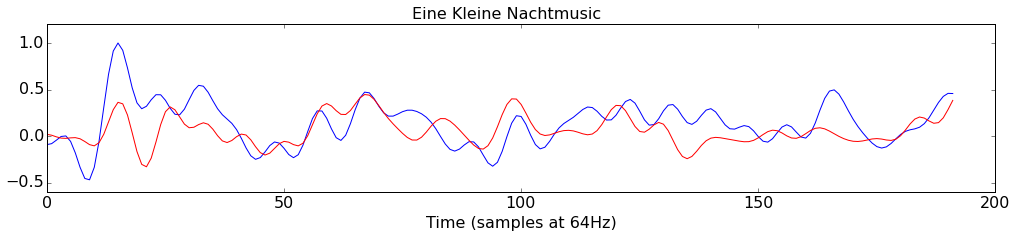
\includegraphics[scale=0.4]{Figures/EineKleineCorrelation}
    \caption{
The time course of component three during perception (blue) and imagination (red) of Eine Kleine Nachtmusic. The correlation between the two time courses is r=0.40 (p$<$0.001).
}
    \label{fig:nachtmusic}
  \end{center}
\end{figure}

\begin{figure}[t]
  \begin{center}
    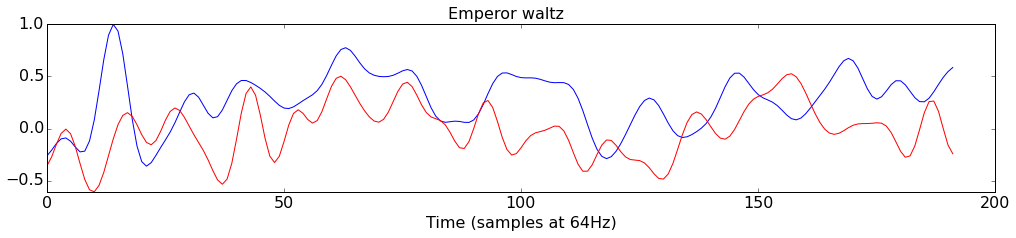
\includegraphics[scale=0.4]{Figures/EmperorCorrelation}
    \caption{
The time course of component three during perception (blue) and imagination (red) of The Emperor Waltz. The correlation between the two time courses is r=0.30 (p$<$0.001).
}
    \label{fig:emperor}
  \end{center}
\end{figure}

\begin{figure}[t]
  \begin{center}
    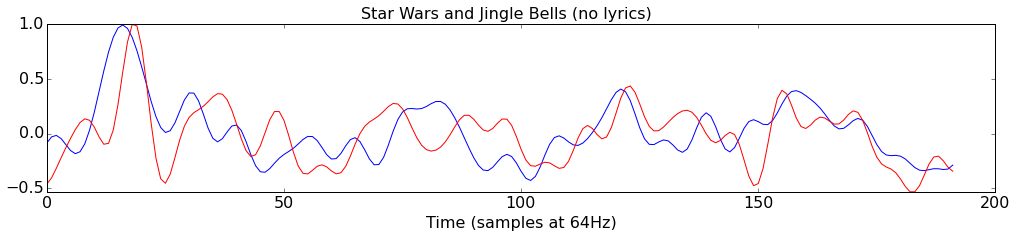
\includegraphics[scale=0.4]{Figures/StarJingle}
    \caption{
The time course of component three during perception (blue) of the Star Wars theme and imagination (red) of Jingle Bells (no lyrics). The correlation between the two time courses is r=0.52 (p$<$0.001).
}
    \label{fig:starjingle}
  \end{center}
\end{figure}

Our inability to accurately classify stimuli using this technique could be caused by our much smaller number of trials which are substantially longer than those used by \cite{schaefer_name_2011}. 
We only had 5 trials per stimulus, ranging from 6.9s to 16s, while Schaefer et al. (2011) collected 145 trials of each of their stimuli each approximately 3s long.
\chapter{Neural Network}
Schaefer \etal \citeyear{schaefer_name_2011} were able to use the unique time course of the component responsible for the most variance to differentiate between stimuli.
With our components we were unable to reproduce this stimulus classification accuracy. 
 
To classify our data, we used a technique from the computer science called an artificial neural network (\ac{ANN}).
A neural network contains one or more layers that process the data.
In these layers, the input is processed by a filter (weight matrix) that is trained using backpropagation \cite{Rumelhart_backpropagation_1986}. 
Our network was optimized for our stimulus classification task and included three processing layers.
The first layer was pre-trained on the perception data using 432 trials (9 subjects x 12 stimuli x 4 trials) and then was not changed during training of the full 3-layer model. 
One trial of each stimulus from each subject's data was left out to be used as the test set for later model testing (108 trials (9 subjects x 12 stimuli x 1 trial) ).
The full explanation of how we arrived at the best model can be found in \cite{stober_ICLR2016} (arXiv:1511.04306).

\section{Layer 1: Similarity Constraint Encoding}
We wanted to find features in the data that were stable across trials and subjects, and also distinguished between classes. 
To identify such features, we used a pre-training strategy called \emph{similarity-constraint encoding}.
% in which the \ac{CAE} is trained to encode relative similarity constraints. 
As introduced by Schultz and Joachims \citeyear{schultz_learning_2004}, a relative similarity constraint $(a,b,c)$ describes a relative comparison of the trials $a$, $b$, and $c$ in the form ``$a$ is more similar to $b$ than $a$ is to $c$.''
Here, $a$ is the reference trial used for this comparison, $b$ is a trial from the same stimulus, and $c$ is a trial from another stimulus.
The number of violated constraints is used as a cost function for learning features of the data that are important for stimulus classification. 
A cost function describes the characteristics of the system that we want to minimize -- in this case we want to minimize the number of violations to the similarity constraint.

To this end, we combined all pairs of trials $(a,b)$ from the same stimulus with all trials $c$ from other stimuli.
During supervised learning, the system was forced to learn features of the data constrained by $a$ and $b$ being more similar than $a$ and $c$. 
For example, we created all possible pairs of trials from the perception of Jingle Bells with lyrics and then combined each of those pairs with all other perception trials.
Each one of these triplets was then processed by the \ac{SCE}. % (under the similarity constraint).
The \ac{SCE} learned features, in this case EEG channel weights, that, when applied to the EEG trials, produced representations of each one of the trials in the triplet. 
The representations were compared using the dot product as a similarity measure. 
Each triplet produced two similarity scores: one comparing $a$ and $b$ (trials from the same stimulus) and one comparing $a$ and $c$ (trials from different stimuli).
Based on our constraint, the similarity score between $a$ and $b$ must be higher than $a$ and $c$.

During training, the number of violated constraints was minimized using backpropagation and stochastic gradient descent with a learning rate momentum \cite{rumelhart1988learning}.
In this scenario, backpropagation allowed the \ac{SCE} to update its learned features (channel weights) to produce representations of the trials that satisfied the constraint. 
To help the \ac{SCE} hone in on the optimal learned features, stochastic gradient descent forced the learned features to be updated in the direction of minimizing the violations of the constraint. 
Learning rate momentum is a method for quickly achieving optimal results. Rather than the features (channel weights) being updated after each triplet was processed, the features were updated after 128 trials had been processed.
%Dropout regularization was used \cite{srivastava2014dropout} to prevent overfitting.
%Dropout regularization is a technique that randomly removes parts of the network during training producing a number of ``thinned'' networks. 
The final features learned by the \ac{SCE} represent those that describe similarities between trials from the same stimulus and differences between trials from different stimuli.  

The spatial representation of the features learned by this \ac{SCE} is visualized in Layer 1 of \autoref{fig:model_W}. 
The coloured areas represent the regions and the electrode weightings that the encoder has determined are optimal for differentiating stimuli.
This representation acts as a spatial filter that processes the raw data.
The 64 EEG channels are reduced to a single data stream of weighted EEG by this filter\footnote{After being processed by the spatial filter we applied a non-linear activation function to the data (a step which generally occurs in all neural network layers).
We used the tanh function here.}. 
\begin{figure}[h] 
  \begin{center}
    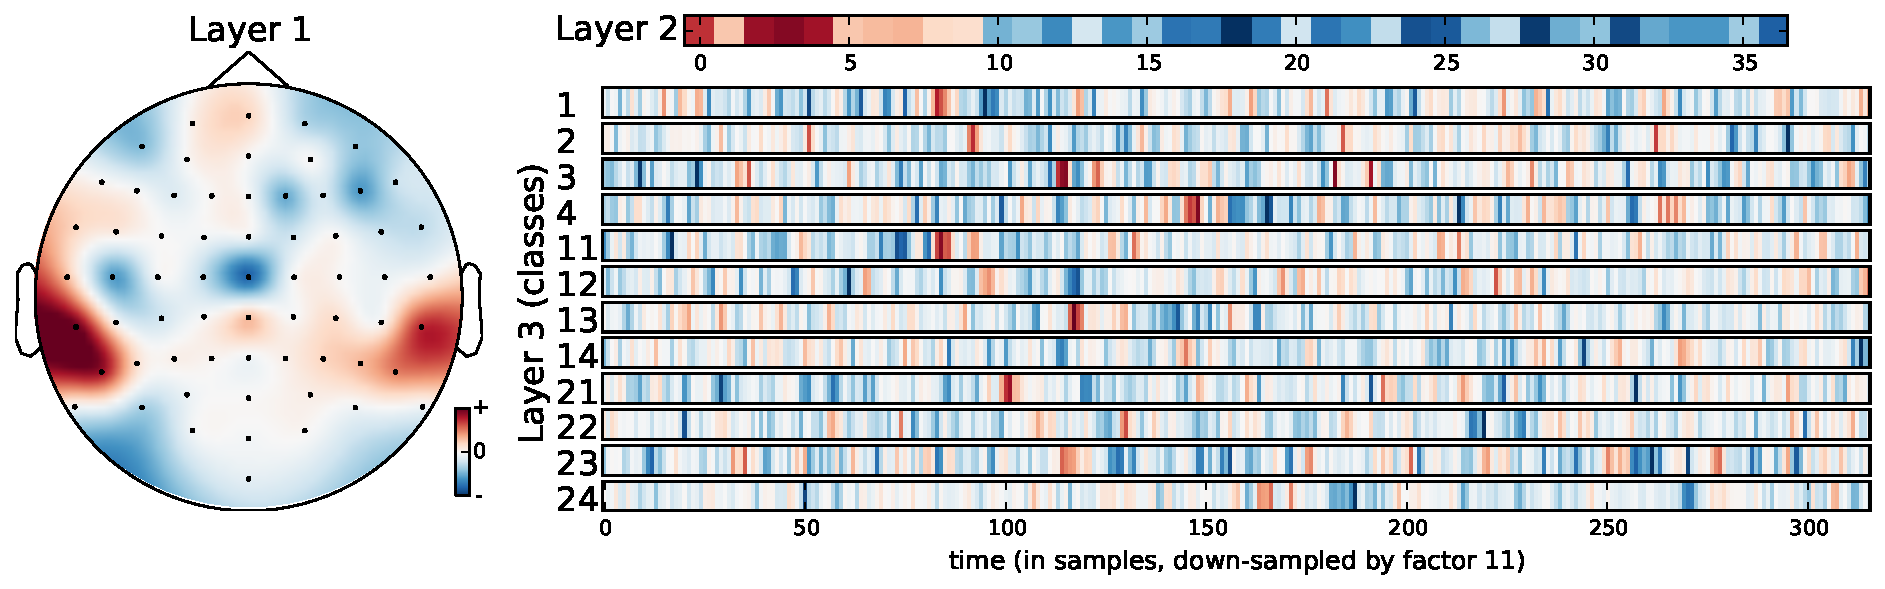
\includegraphics[width=\textwidth,keepaspectratio=true]{Figures/model_W}
%   \\\vspace{-0.8em}
    \caption{Visualization of our neural network, which processes raw EEG at a sampling rate of 512\,Hz.
    Layer 1 was pre-trained using similarity-constraint encoding and is a spatial representation of EEG electrode weights. Layer 2 is a 37 sample long temporal filter. Layer 3 shows the compressed representations of the raw EEG data. The numbers are the ID numbers of the stimuli found in \autoref{tab:stimuli_information}. The colours are an indication of the weighting decided on by the model. We can interpret the intense red and blue colours as being more important for stimulus classification than the white areas.}
    \label{fig:model_W}
  \end{center}
%  \vspace{-1em}
\end{figure}
\section{Layer 2: Temporal Filter \& Layer 3: Templates}
Layers two and three were trained together with supervised learning and optimized by backpropagation through the entire model with a cost function to minimize classification error.
The single data stream output from layer one entered the second layer where it was processed the filter and pooled with a subsampling factor of 11.
This produced a compressed representation of the original EEG data.

To find the optimal parameters (learning rate, filter size, etc.) for our neural network, we employed a 9-fold cross validation scheme by training on the data from 9 subjects (384 trials) and validating on the remaining subject (48 trials).
The cross-validation was done within the training set. %This process created optimized, compressed representations of the EEG data for each stimuli.
The final versions of layer 2 and 3 seen in \autoref{fig:model_W} are an average of the model parameters over all 9 folds.
Layer 2 is the filter that processes the data stream from layer 1, and layer 3 is made up of the optimized, compressed representations of the original EEG data for each stimulus.
\section{Full model explanation}
The classification accuracy of the model was then tested with the test set of 108 trials. 
Each trial in the test set was processed by the filters in layer 1 and layer 2. 
The resulting compressed representation (the output from layer 2) of the test trial was compared against each of the optimized representations in layer 3 of the model.
The dot product of the test trial's representation was taken with each of the optimized layer 3 representations.
This produced 12 values (one for each stimulus) that described the similarity of the test trial's representation with each of the optimized representations. 
Using the dot product as a similarity measure, the test trial was given the label of the stimulus whose representation it was most similar to. 
%\chapter*{Classification}
\addcontentsline{toc}{chapter}{Classification}
Schaefer \etal \cite{schaefer_name_2011} were able to use the unique time course of the component responsible for the most variance to differentiate between stimuli.
Analyzing our components we have not yet been able to reproduce this significant stimulus classification accuracy. 
This could be caused by our much smaller number of trials which are substantially longer than those used by \cite{schaefer_name_2011}. 
On average we used \hl{X number of} trials in our analysis, while Schaefer et al. (2011) collected 145 trials of each of their stimuli.

We then attempted a different approach to classification using machine learning techniques. This approach facilitates better pattern learning by adapting components linked across subjects but that are also specific to each individual subject. 
We trained a \ac{CAE} as described in \cite{masci_stacked_2011} and implemented using pylearn2 \cite{goodfellow_pylearn2_2013}.
%CAEs are a special variant of a \ac{CNN} that encode their input using convolution into a compressed internal representation which is then decoded using de-convolution into the original space trying to minimize the reconstruction error. 
%Such a neural network can be used to learn a meaningful but compressed representation of the data. 
In this case the 64 \ac{EEG} channels were reduced to four combined channels -- each computed by a separate convolution filter. 
%These filters are very similar to the components produced in \ac{PCA} and \ac{ICA}. 
%The difference is the objective that is used to compute these components. 
%The \ac{CAE} filters aim to minimize the \ac{MSRE} using stochastic gradient descent over mini-batches rather than the orthogonality or independence criteria used in \ac{PCA} and \ac{ICA} respectively. 
\subsection*{Perception Classification Results}
First the \ac{CAE} was trained on all trials in the perception condition. The learned filter weights were then used as initialization values to create individual \ac{CAE}s specific to each participant.
The filters can be seen in \autoref{fig:components}. 
Minor differences between subjects can be seen. 

\begin{figure}[t]
  \begin{center}
    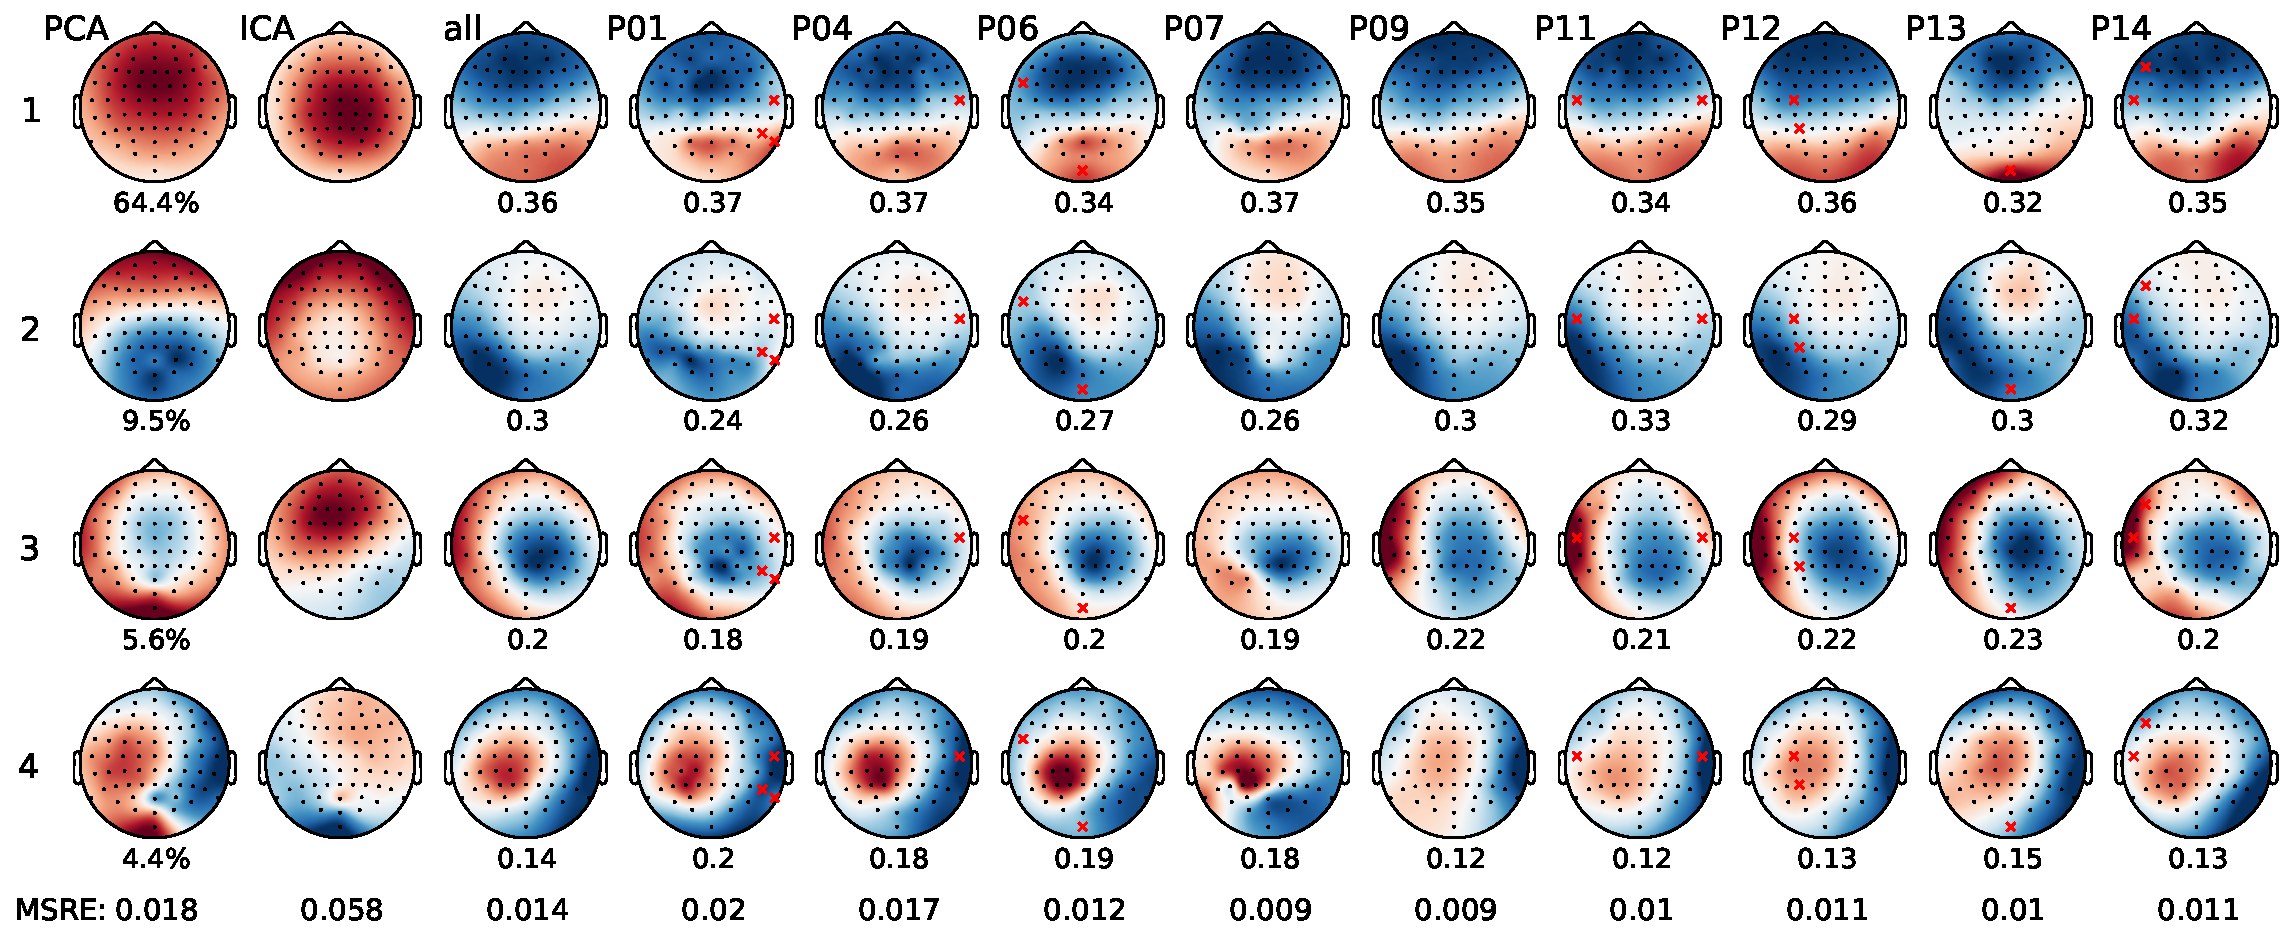
\includegraphics[width=\columnwidth,keepaspectratio=true]{Figures/topoplots_all.pdf}
    \caption{
Topographic map visualization of the EEG channel weights for the top 4 signal components derived from the perception trials. The leftmost two columns show the top 4 principal components (explaining over 87\% of the variance in total) and the corresponding independent components computed using extended Infomax ICA. The remaining columns show the weights learned by the convolutional auto-encoder for all subjects combined (third column) and all individual subjects labeled P01 to P14 accordingly. Numbers below the plots refer to the percentage of explained variance for principal components and the normalized biases for the filters of the convolutional auto-encoder respectively. Noisy EEG channels that were removed and interpolated are marked by red X?s. For subjects P09 to P14, mastoid channel referencing was applied. Values at the bottom of each column refer to the mean squared reconstruction error (MRSE) per sample.
}
    \label{fig:components}
  \end{center}
\end{figure}

We used the data from the learned components to train simple \ac{CNN}s with a single convolution layer and a \hl{DLSVM output layer} \cite{tang_deep_2013} on two classification tasks: stimulus identification (12 classes) and time-signature recognition (2 classes). 
We trained the CNN on 60\% of the trials. This same training set was used to train the \ac{CAE} prior to the \ac{CNN} training. 
The best model was selected using a validation set (20\% of trials) and it was evaluated on a test set (20\% of trials). 
\hl{We used dropout regularization} \cite{hinton_improving_2012}, momentum, and a linear learning rate decay over epochs.
A simple \ac{CNN} that used 16 [1x4]-convolution filters (over 1 sample in all 4 component activation channels) obtained 65.8\% (p=0.05) accuracy on the binary time-signature classification task. 
A CNN using 1 [16x4]-convolution filter (over 250ms in all 4 component activation channels with pooling for 140ms-windows and 5x sub-sampling obtained 19.5\% (p=0.001) on the 12 class stimulus recognition task. 
Significance values were determined by using the cumulative binomial distribution to estimate the likelihood of observing a given classification rate by chance.

\subsection*{Imagination Classification Results}
Imagination results from CNN. 

Table to summarize all results? 

\section{Results}
First, we tested the model with the perception data. 
Significance values were determined by using the cumulative binomial distribution to estimate the likelihood of observing a given classification rate by chance \cite{Combrisson2015}. 
Using the cumulative binomial distribution allows us to determine the number of observations that are correctly classified by chance with respect to the number of observations.
Our model was able to classify the 12-classes (12 stimuli listed in \autoref{tab:stimuli_information}) with a 28.7\% accuracy rate (chance = 17.59\%) at a significance level of p=0.001.
\autoref{fig:model_W_confusion} is a confusion matrix which shows the classification results for each stimulus.
\begin{figure}[htb] 
  \begin{center}
    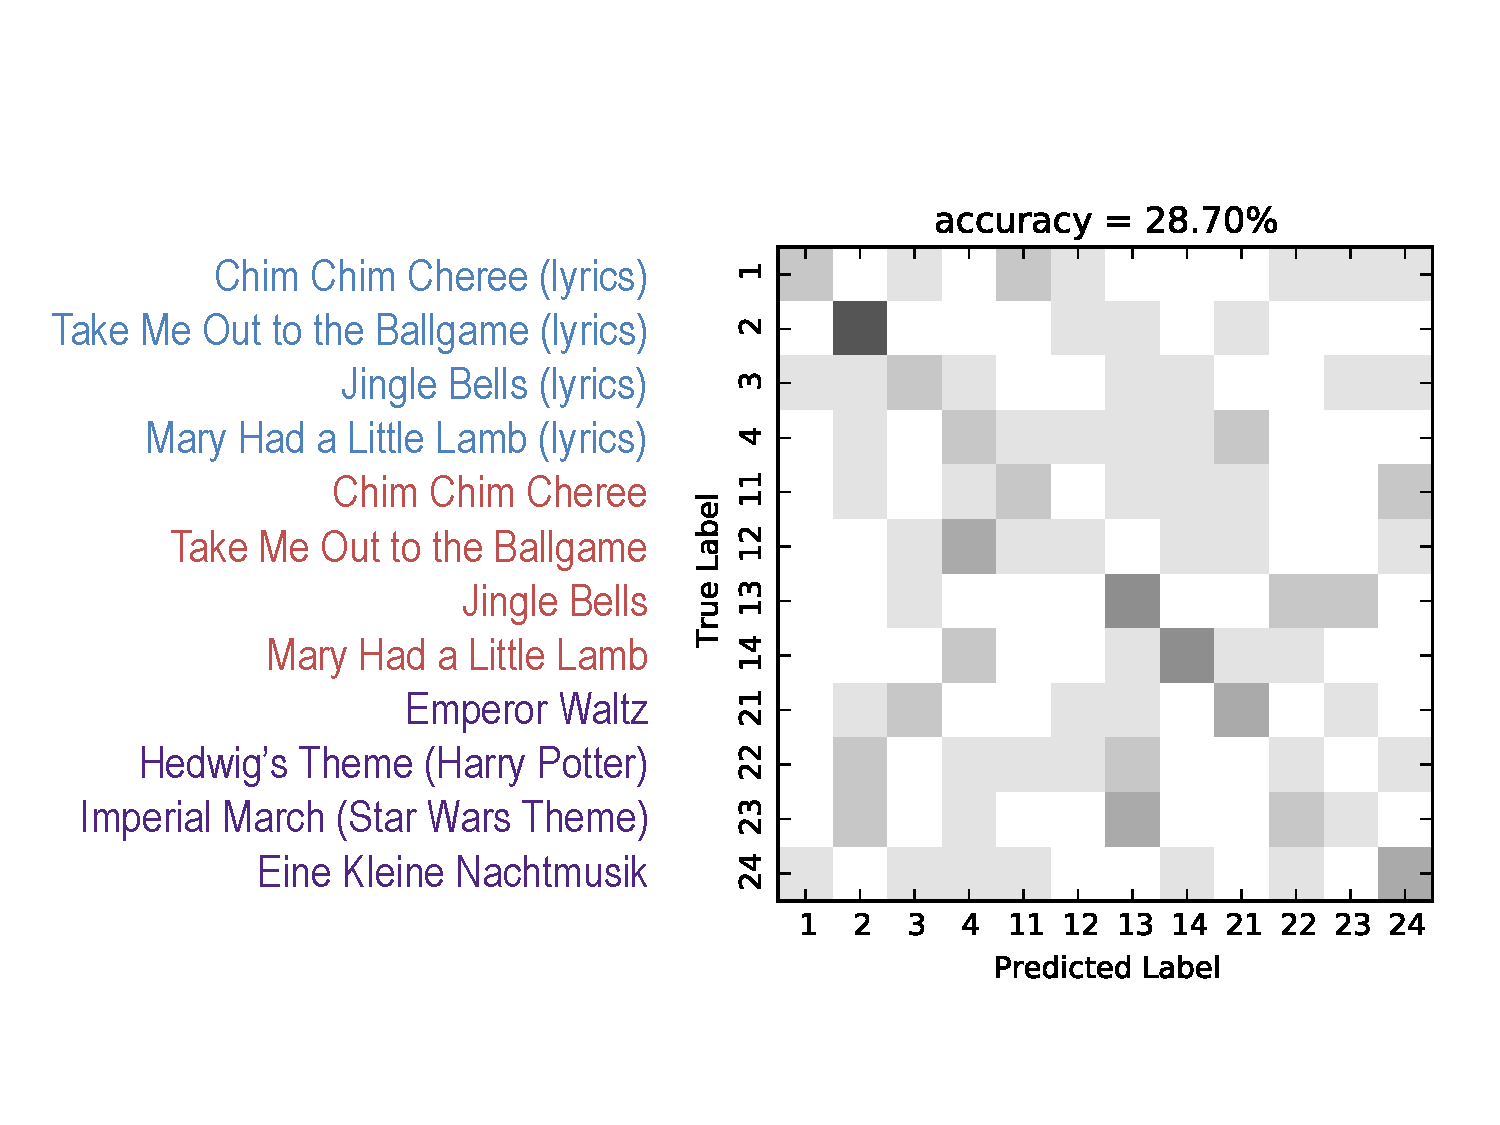
\includegraphics[width=.75\textwidth,keepaspectratio=true]{Figures/model_W_confusion-512}
   \\\vspace{-0.8em}
    \caption{12-class confusion matrix for perception data. The numbers are the ID numbers of the stimuli found in \autoref{tab:stimuli_information}. Colour indicates the number of times a true label was classified as a predicted label with darker colours indicating more classifications.}
    \label{fig:model_W_confusion}
  \end{center}
%  \vspace{-1em}
\end{figure}
From the confusion matrix we can see that some stimuli were more accurately classified than others. 
Stimulus 2 (Take Me Out to the Ballgame with lyrics) is the most accurately classified. 
Stimuli 13 and 14 are also accurately classified, but some confusion with their lyric counterparts (stimuli 3 and 4) can be seen.
Confusion between lyric and non-lyric pairs can also be seen with stimulus 1 being classified as stimulus 11.

To further investigate which pairs of stimuli the classifier could distinguish best, we put all combinations of paired stimuli through our classifier.
This resulted in the series of binary confusion matrices in \autoref{fig:model_W_binary_confusion} that show us that some pairs of stimuli are more easily differentiated than others. 
\begin{figure}[htb] 
  \begin{center}
    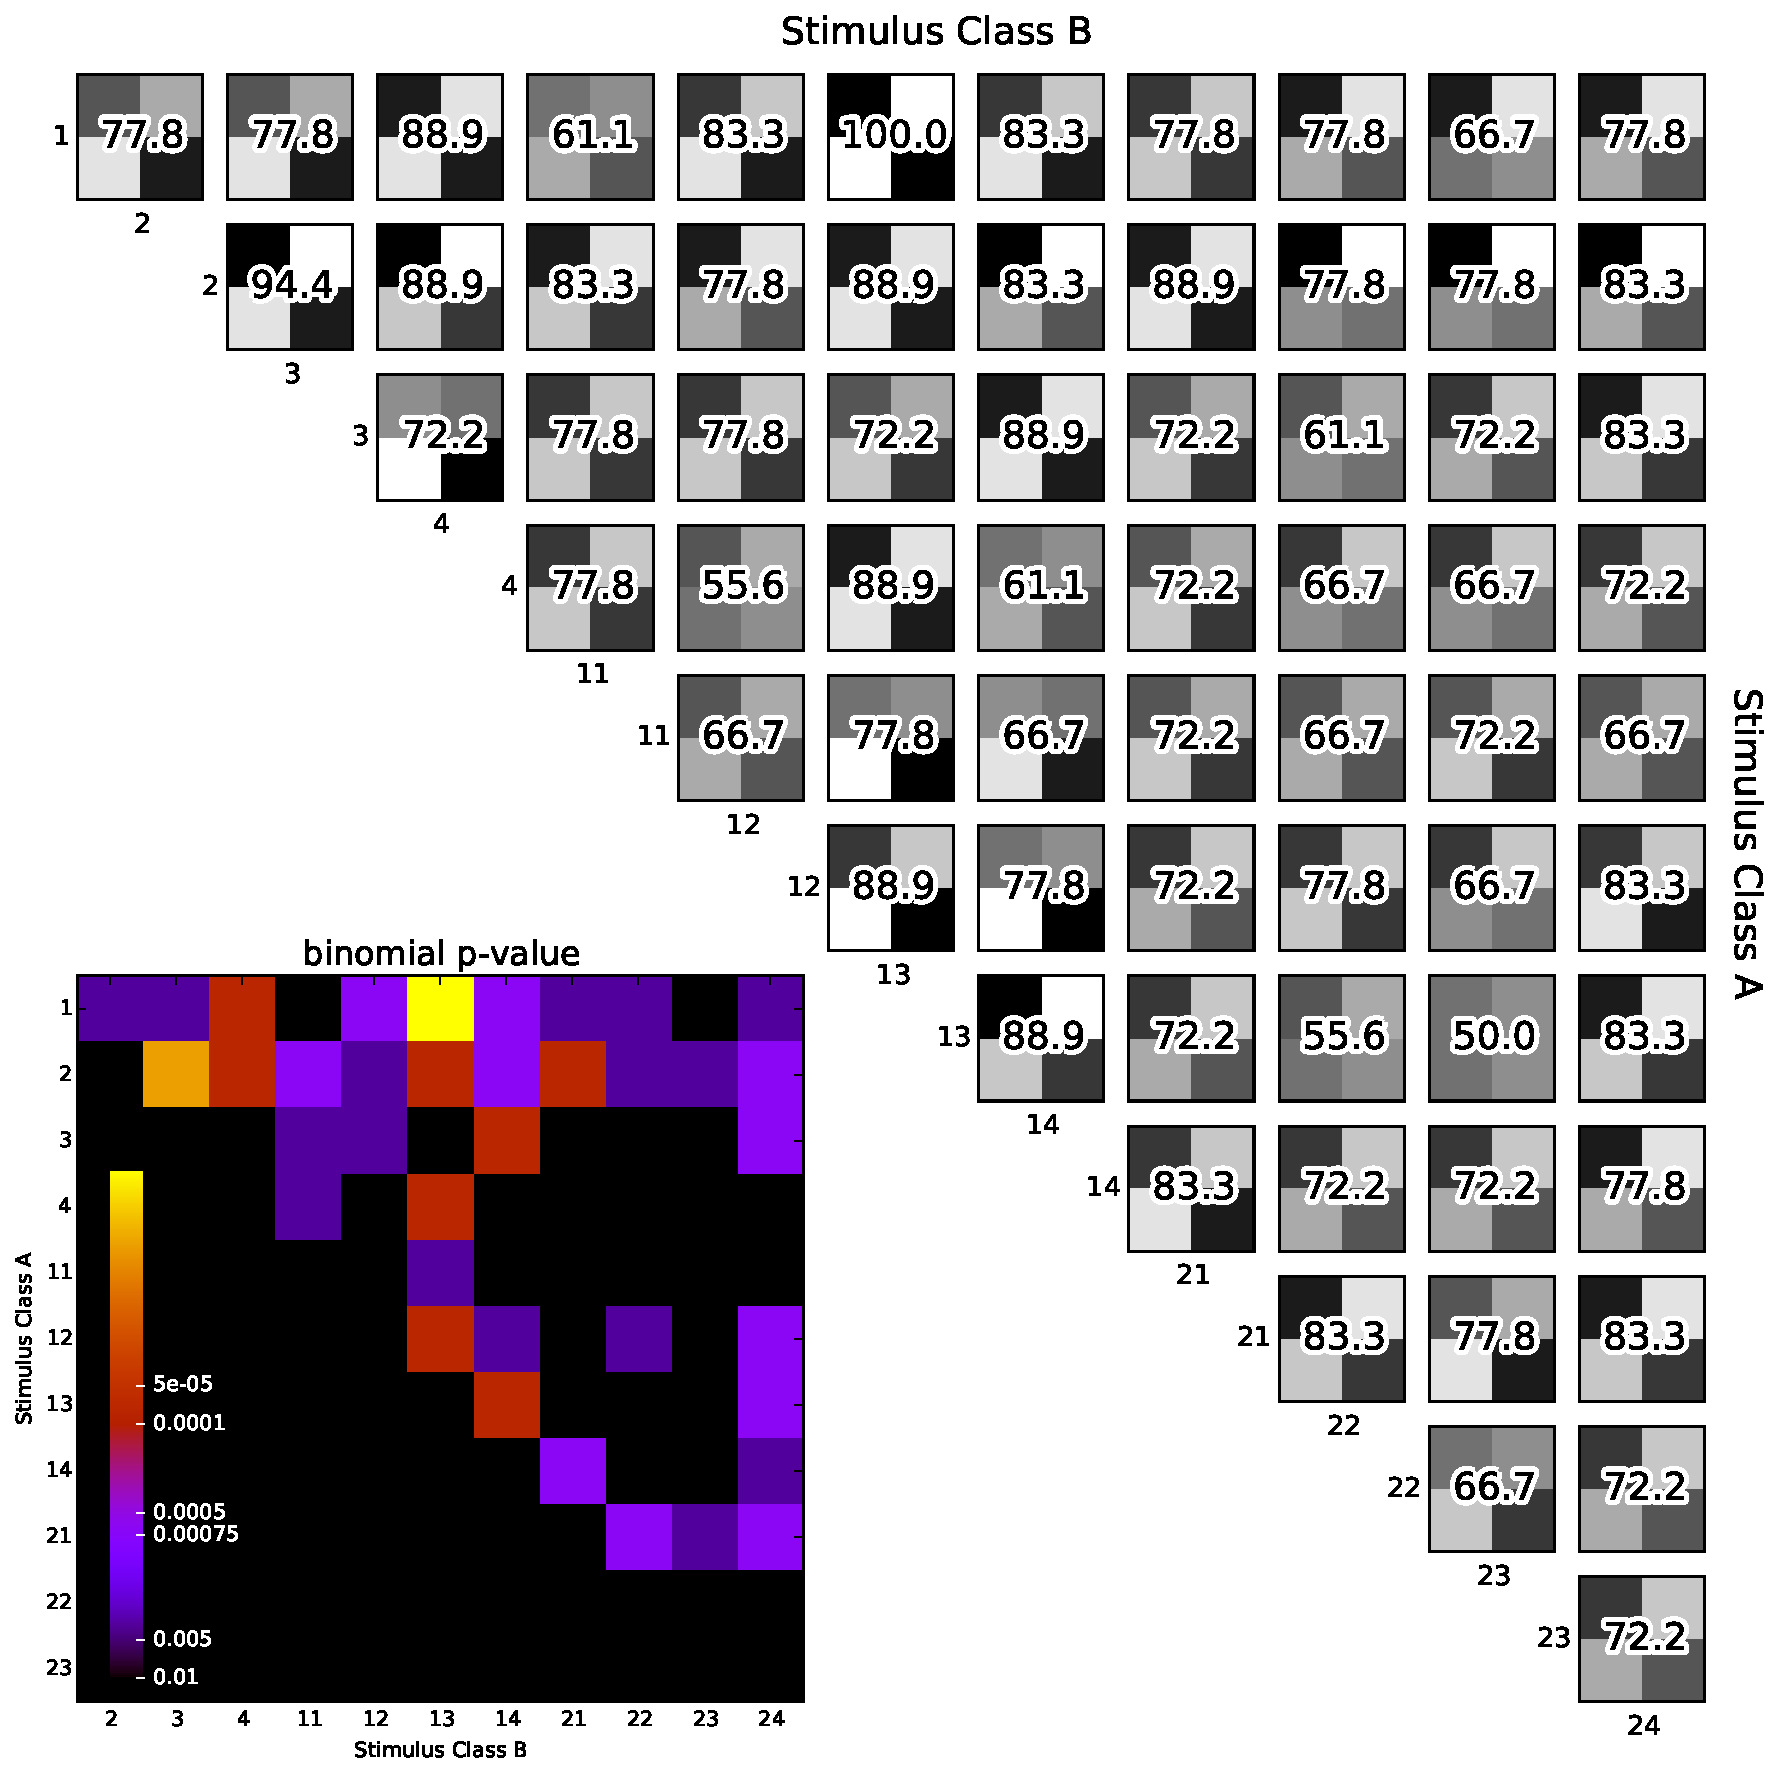
\includegraphics[width=.8\textwidth,keepaspectratio=true]{Figures/model_W_binary_confusion-512}
   \\\vspace{-0.8em}
    \caption{Binary confusion matrices for perception data.
    The inset shows the p-values determined by using the cumulative binomial distribution to estimate the likelihood of observing the respective binary classification rate by chance. The significance threshold was bonferroni corrected to $alpha$ =  0.05/66 = 7.5e-04}
    \label{fig:model_W_binary_confusion}
  \end{center}
  \vspace{-1em}
\end{figure}
For example: Chim Chim Cheree with lyrics is classified correctly 100\% of the time when paired with Jingle Bells without lyrics.
Within each binary confusion matrix chance is 66.67\% (alpha = 0.05).
The statistical significance (p-value) of each of the comparisons is visualized in the figure's inset. 
%Most of the binary comparisons are classified correctly at a statistically significant level (p$<$0.05). 

The imagination data was then tested on the same model (i.e. there was no additional training using the imagination data). 
The model was not able to classify the 12 stimuli from the EEG data collected during music imagination. 
\autoref{fig:model_W_confusion_cond2} is a confusion matrix which shows the imagination classification results at 7.41\% (below chance = 12.96\%, alpha = 0.05). 
As can be seen in the figure, there is no clear pattern to the confusion indicating that the system was not making classification errors in a systematic way. 
\begin{figure}[htb] 
  \begin{center}
    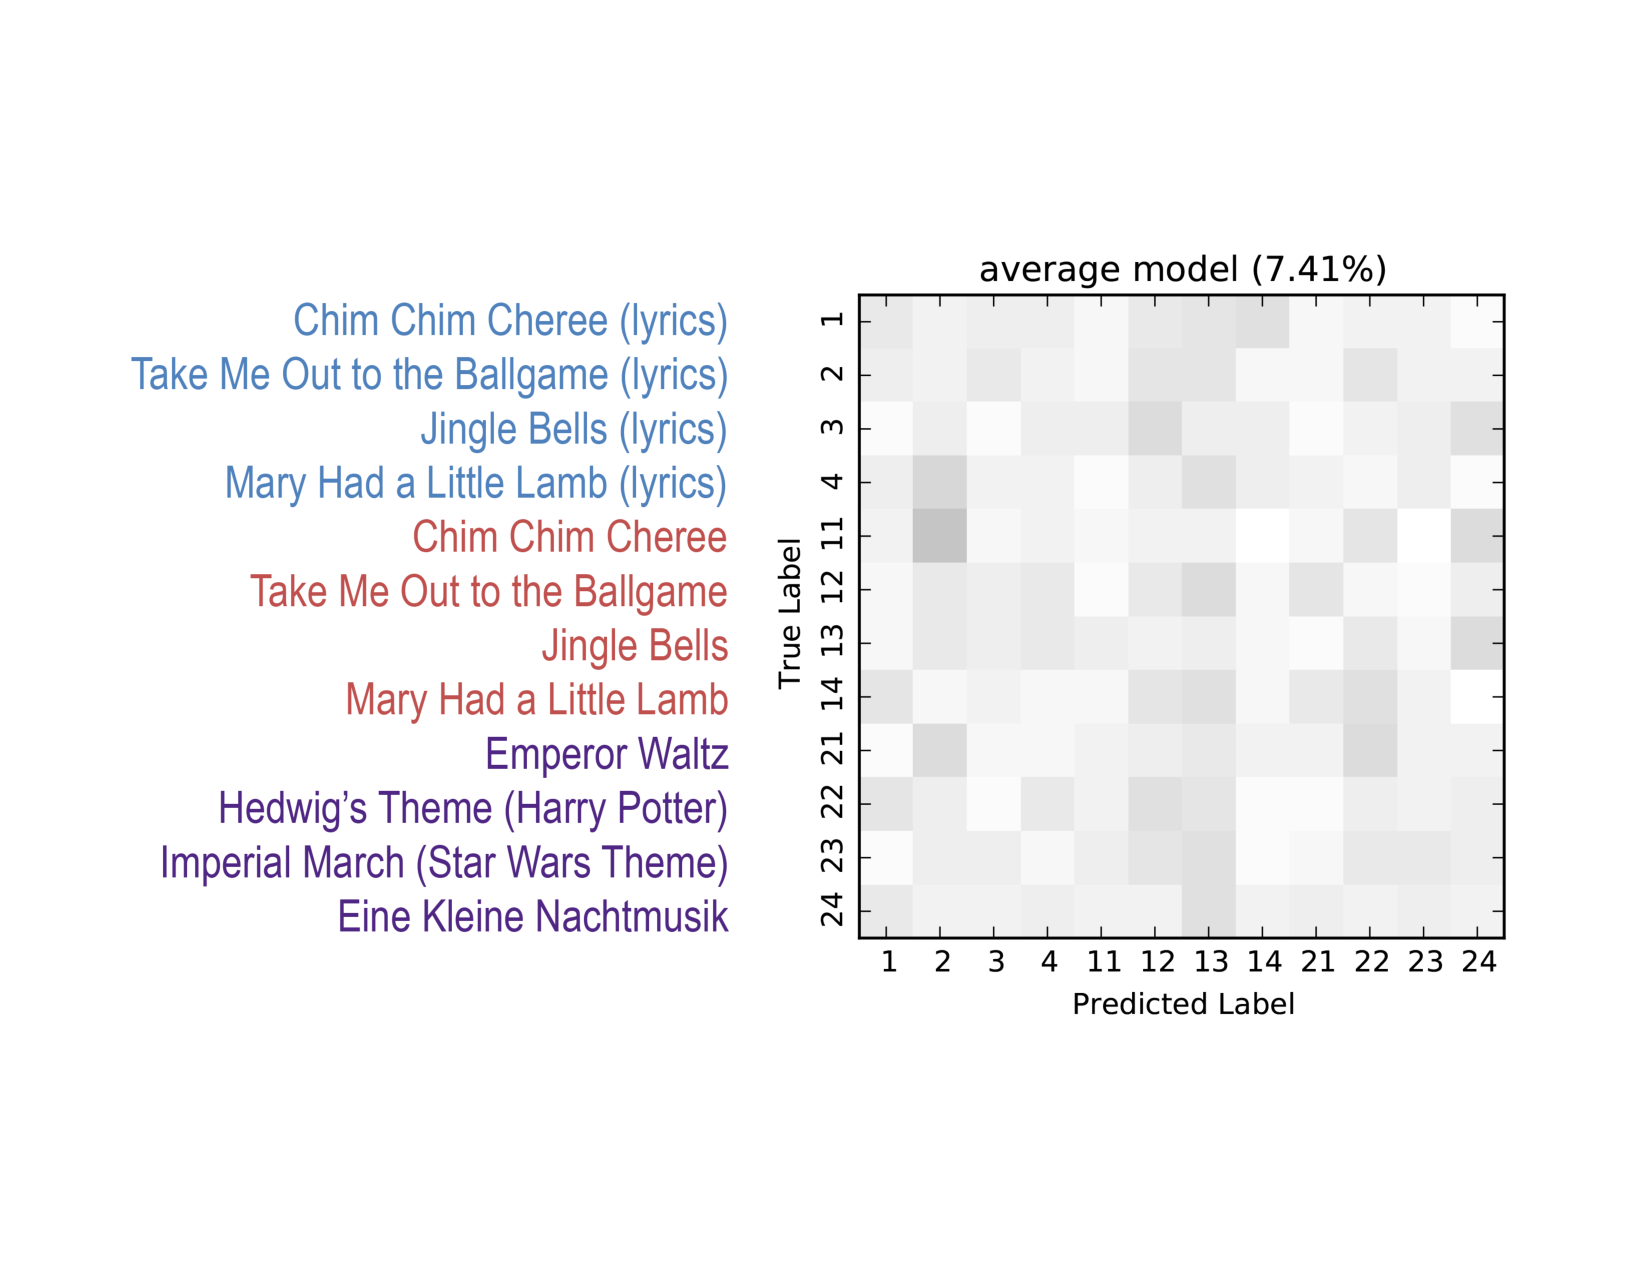
\includegraphics[width=.83\textwidth,keepaspectratio=true]{Figures/model_W_confusion_cond2}
   \\\vspace{-0.8em}
    \caption{12-class confusion matrix for imagination data. The numbers are the ID numbers of the stimuli found in \autoref{tab:stimuli_information}. Colour indicates the number of times a true label was classified as a predicted label with darker colours indicating more classifications.}
        \label{fig:model_W_confusion_cond2}
  \end{center}
  \vspace{-1em}
\end{figure}

We investigated whether there were pairs of imagined stimuli that the classifier could distinguish.
\autoref{fig:model_W_binary_confusion_cond2} shows the binary confusion matrix.
None of the stimulus pairs were classified at a statistically significant level. 

\begin{figure}[h] 
  \begin{center}
    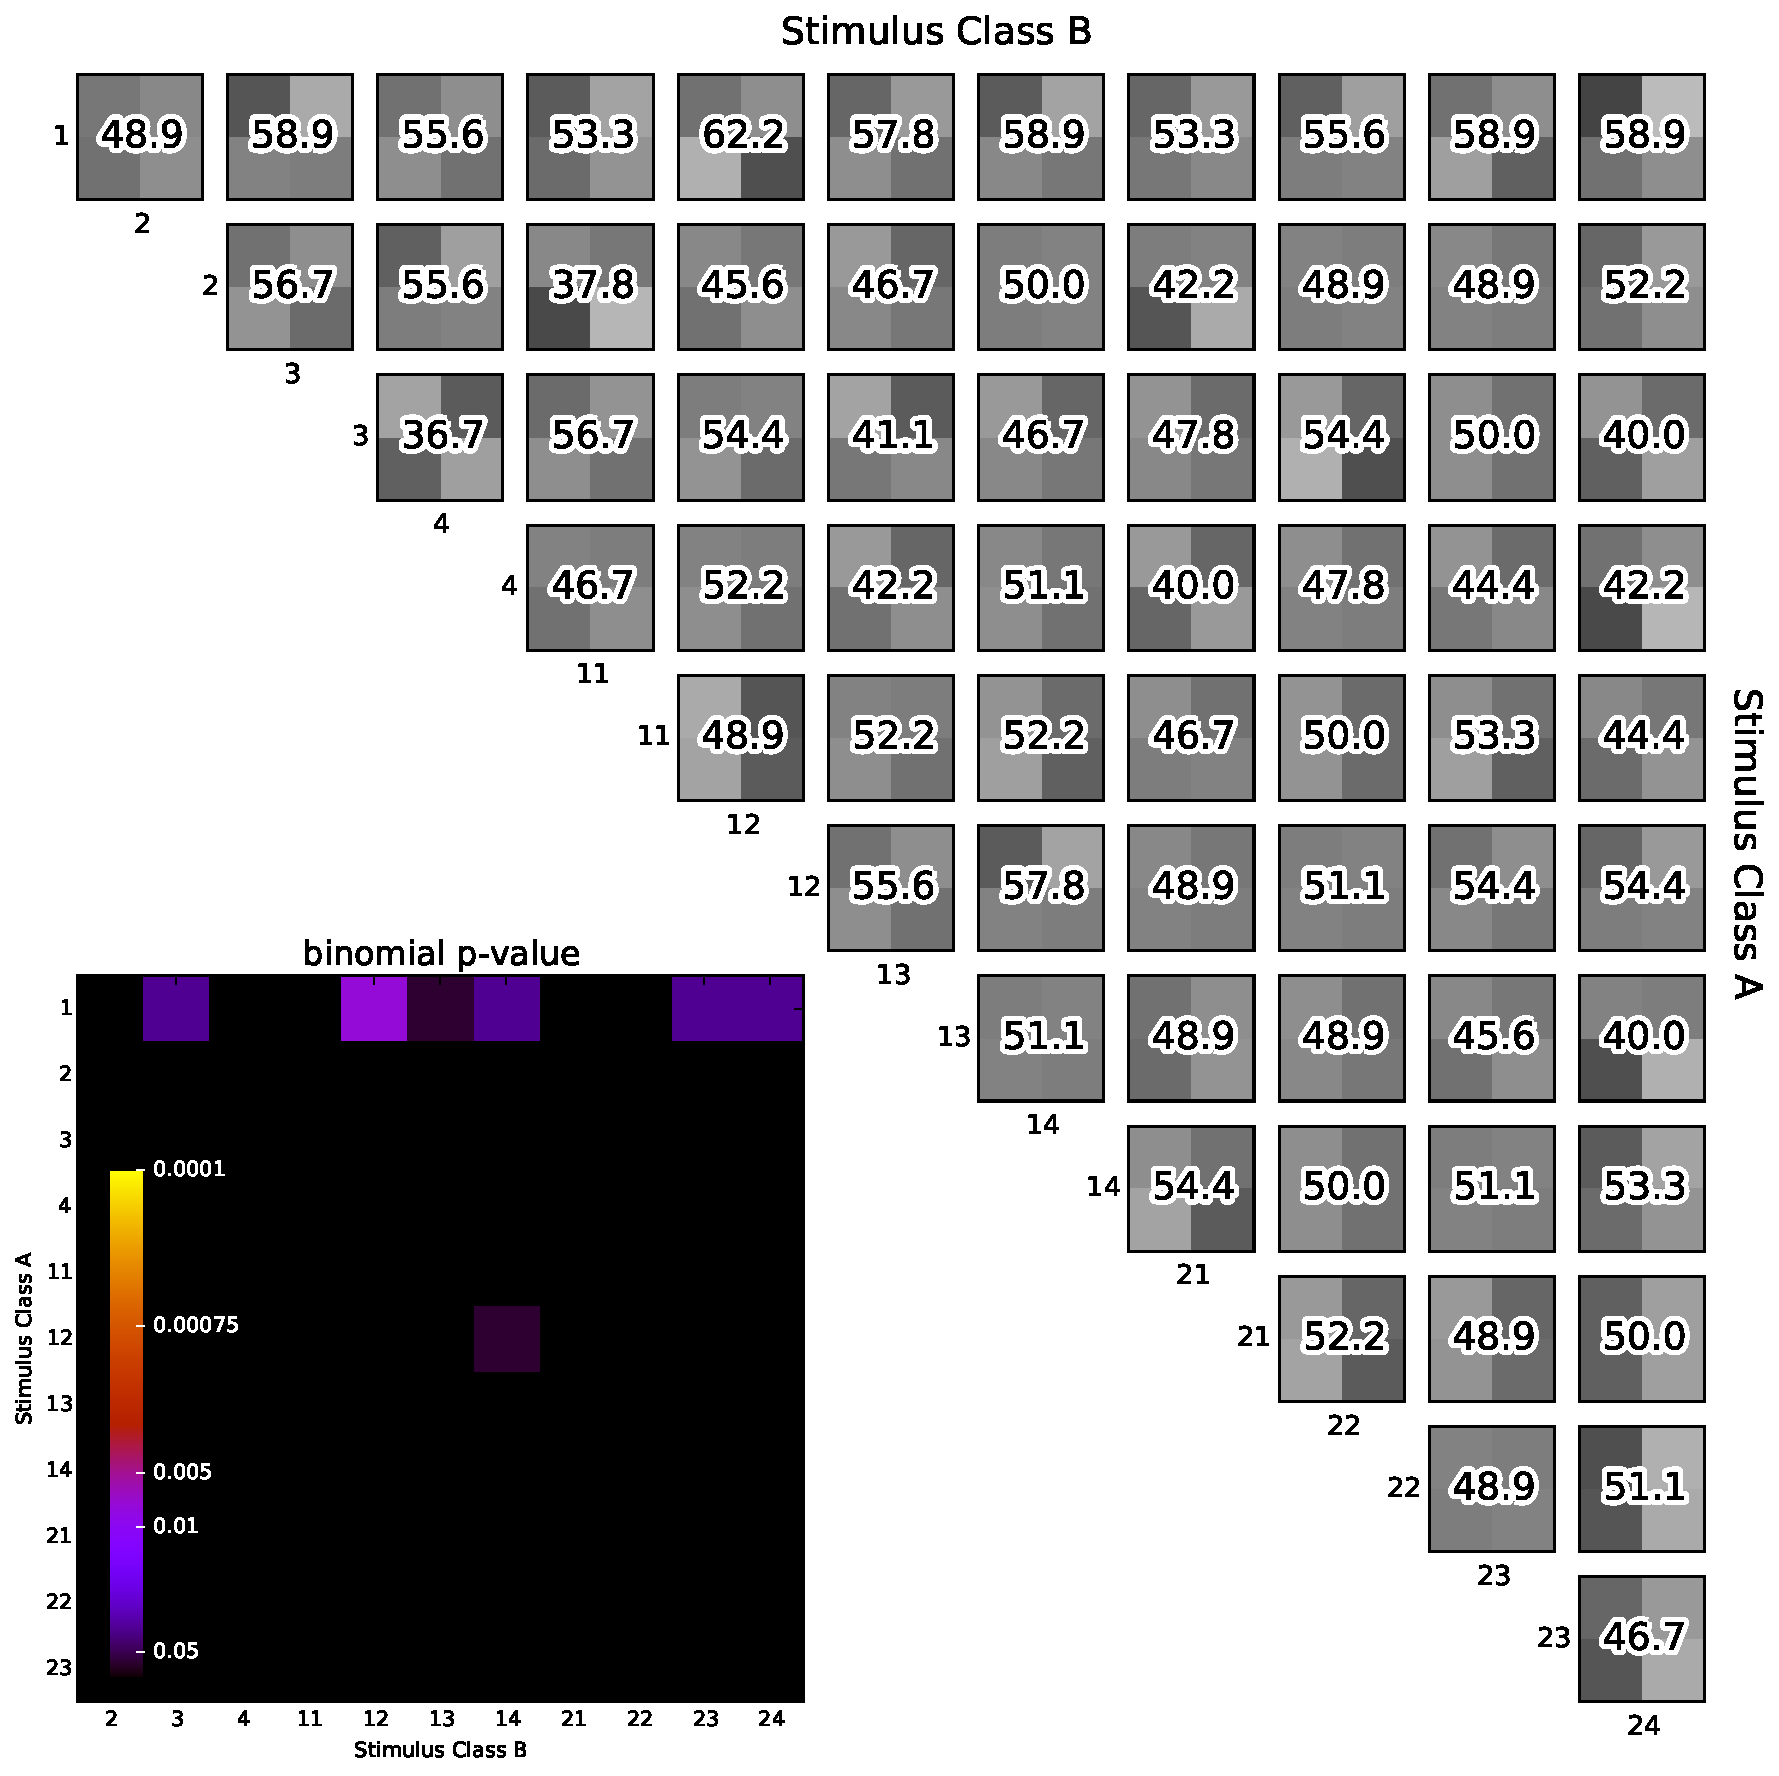
\includegraphics[width=.75\textwidth,keepaspectratio=true]{Figures/model_W_binary_confusion_cond2}
   \\\vspace{-0.8em}
    \caption{Binary confusion matrices for imagination data.
    The inset shows the p-values determined by using the cumulative binomial distribution to estimate the likelihood of observing the respective binary classification rate by chance. The significance threshold was bonferroni corrected to $alpha$ =  0.05/66 = 7.5e-04}
    \label{fig:model_W_binary_confusion_cond2}
  \end{center}
  \vspace{-1em}
\end{figure}
\newpage
\section{Discussion}
The neural net does not give us information about what characteristics from the EEG it used to classify the stimuli, and it is difficult to interpret from the results what signals the brain is producing that allow this classification to occur. 
In layer 3 of \autoref{fig:model_W} we see compressed representations of the EEG data for each stimulus. 
One characteristic of these representations is the dark red vertical bands that stand out from the rest of the time course. 
These red bands indicate time periods that the neural net has identified as being important for classifying the stimuli.
When taking a closer look, we see that these bands occur at the same time point for lyric/non-lyric pairs of stimuli. 
For example, the darkest red band in stimulus 1 (Chim Chim Cheree with lyrics) appears at a very similar time point as the darkest red band in stimulus 11 (Chim Chim Cheree without lyrics).
A similar pattern can be seen for stimuli 2/12 and 3/13.
Upon investigation of the audio of the stimuli at these time periods, there were no characteristics (e.g. lyric repetition, important music moments, end of phrases, change in dynamics, etc.) that stood out as driving these moments to be labeled as important.
These red bands may represent a cognitive process, such as recognition, that occurs at these time points during perception of the stimuli. 
To investigate this possibility, we ran a follow-up behavioural experiment asking participants to indicate when they consciously recognized each stimulus. 
This experiment is described in the next section.

The results of our neural net show that some stimuli are better classified than others, and some pairs of stimuli are more easily differentiated. 
To investigate whether the neural net is relying on a process similar to that which humans might employ, we ran a follow-up experiment asking participants to rate the similarity of pairs of stimuli. 
The results will tell us whether the neural net confuses songs that humans rate as similar. 
\chapter*{Behavioural Experiment}
\addcontentsline{toc}{chapter}{Behavioural}
%In order to investigate whether the deep learning neural net was identifying characteristics of the music that humans can consciously identify we ran a followup behavioural experiment. 
\subsection*{Participants}
9 participants (4 male), aged 22-28, with normal hearing and no history of head injuries took part in this study. Six participants had formal music training (2-15 years), and four of the participants played instruments regularly at the time of data collection. On average participants listened attentively to music 1.5 hours per day and had music playing in the background for 3.6 hours per day. 
\subsection*{Procedure}
The 12 stimuli used were the same songs as those used in the original experiment (See \autoref{tab:stimuli_information}.)
The experiment had two parts and lasted about 50 mins.
First, participants listened to each of the 12 stimuli and pressed a button when (and if) they recognized the piece of music.
The timing of their key press was recorded. 
During the second part of the experiment participants were presented with all possible paired combinations of stimuli (78 pairs). 
They listened to the first song followed immediately by the second and then rated how similar they felt the two songs sounded on a scale from 0-100 (0=the songs sound nothing alike, 100=the songs sound exactly the same).
Participants were asked to focus on how generally similar the two songs sounded and not to worry about being correct.

\subsection*{Results}
In order to determine whether the periods of time highlighted by the neural net in layer 3 of \autoref{fig:model_W} are representative of a moment of recognition we collected the average time at which people recognize these musical pieces (\autoref{fig:RecognitionTime}). 
From these results it does not look like the highlighted time periods from layer 3 of the neural net are related to the moment at which people recognize the piece of music. 

\begin{figure}[h] 
  \begin{center}
%    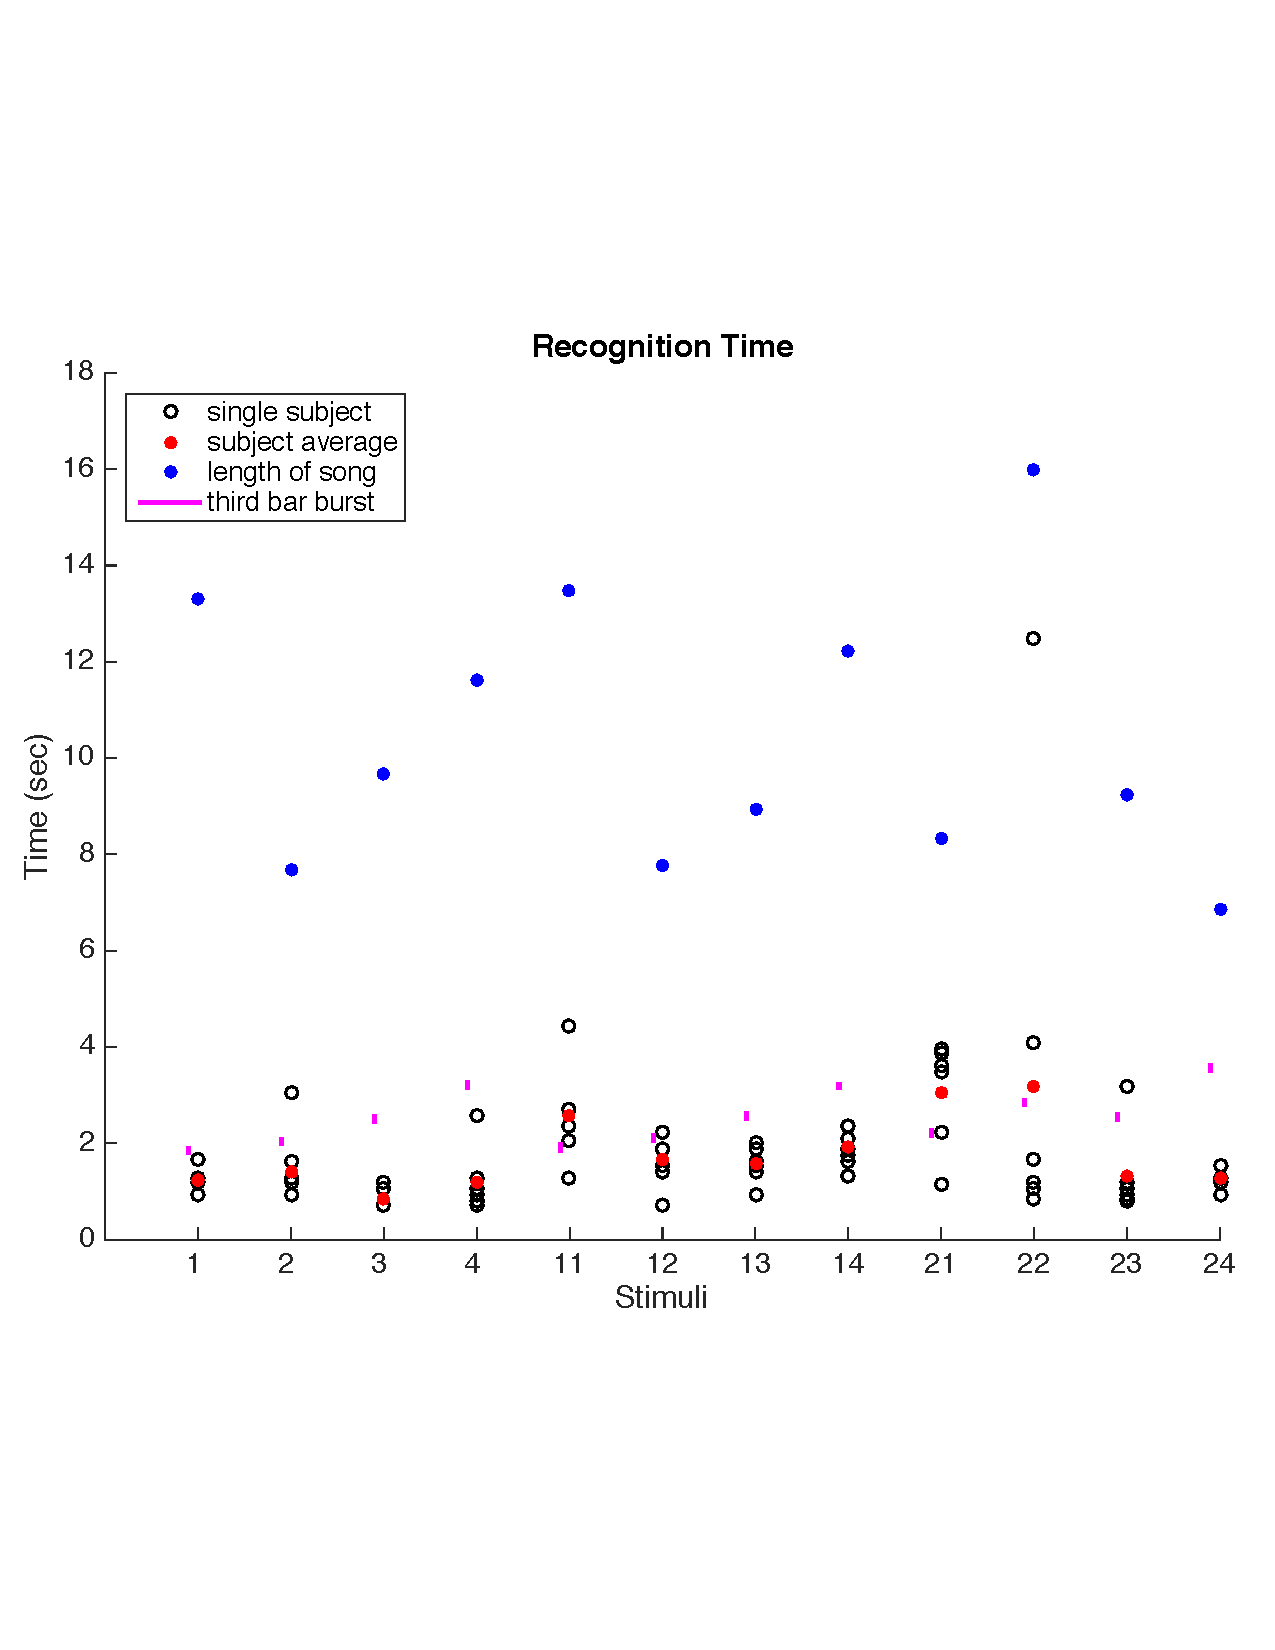
\includegraphics[width=\textwidth,keepaspectratio=true]{Figures/RecognitionTimeGraph}
        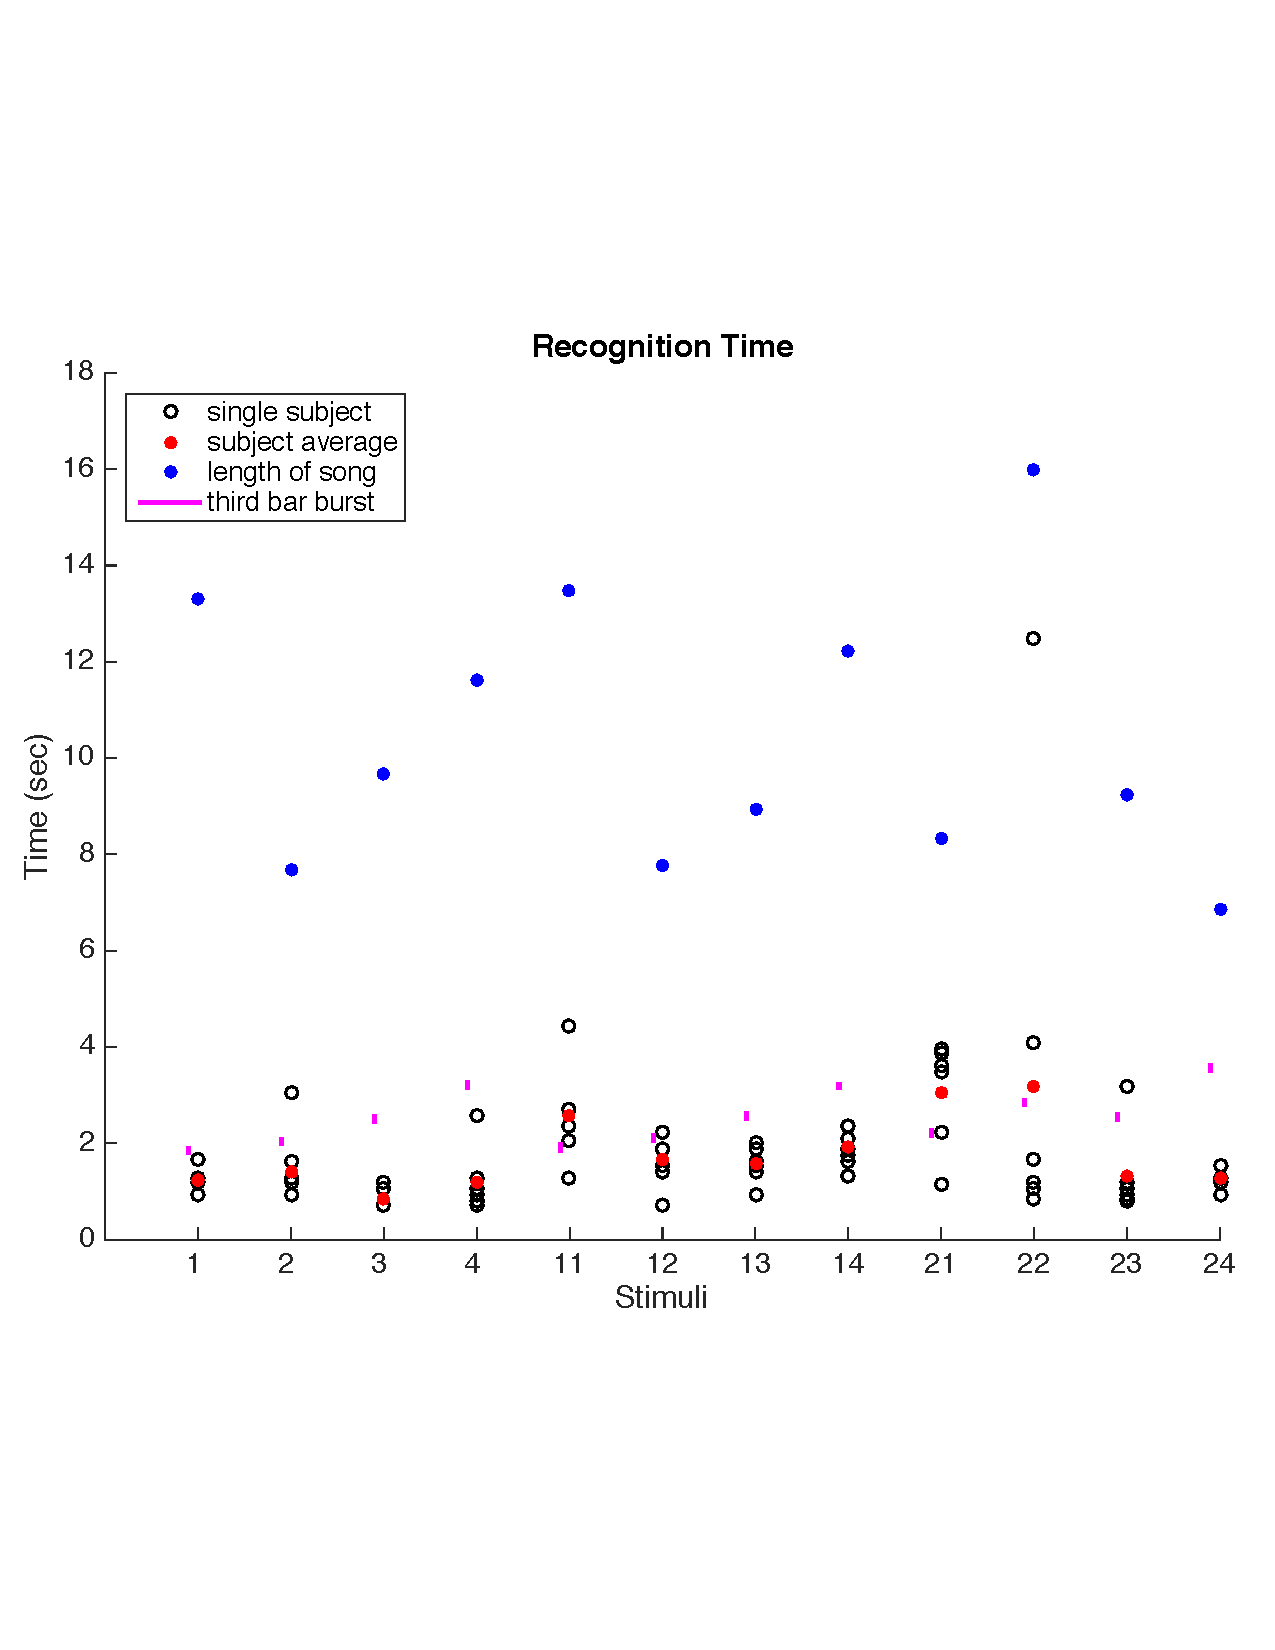
\includegraphics[scale=0.7]{Figures/RecognitionTimeGraph}
%   \\\vspace{-0.8em}
    \caption{Average time it takes for participants to recognize these stimuli (red). Individual data is shown in black and song length is shown in blue. The magenta bars indicate the highlighted time periods from layer three in the neural net (\autoref{fig:model_W_confusion}).}
    \label{fig:RecognitionTime}
  \end{center}
%  \vspace{-1em}
\end{figure}

The second part of the experiment asked participants to give similarity ratings of pairs of songs in order to determine whether the neural net confuses songs that humans rate as similar. 
\autoref{fig:Similarity} shows the similarity rating results. 
As expected, participants are close to perfect at identifying identical songs. 
Lyric/non-lyric pairs of songs were also rated as highly similar and that is seen in the four, dark squares parallel to the diagonal.

The values seen in \autoref{fig:model_W_binary_confusion} can be interpreted as ``dissimilarity'' scores, so we took their inverse (100 - score) to produce similarity scores and correlated this matrix with the average similarity ratings given by our participants.
A correlation of r=0.0012 was calculated (p$>$0.05).
This lack of correlation indicates that the neural net is doing something different than humans when determining similarities between stimuli. 

\begin{figure}[h] 
  \begin{center}
%    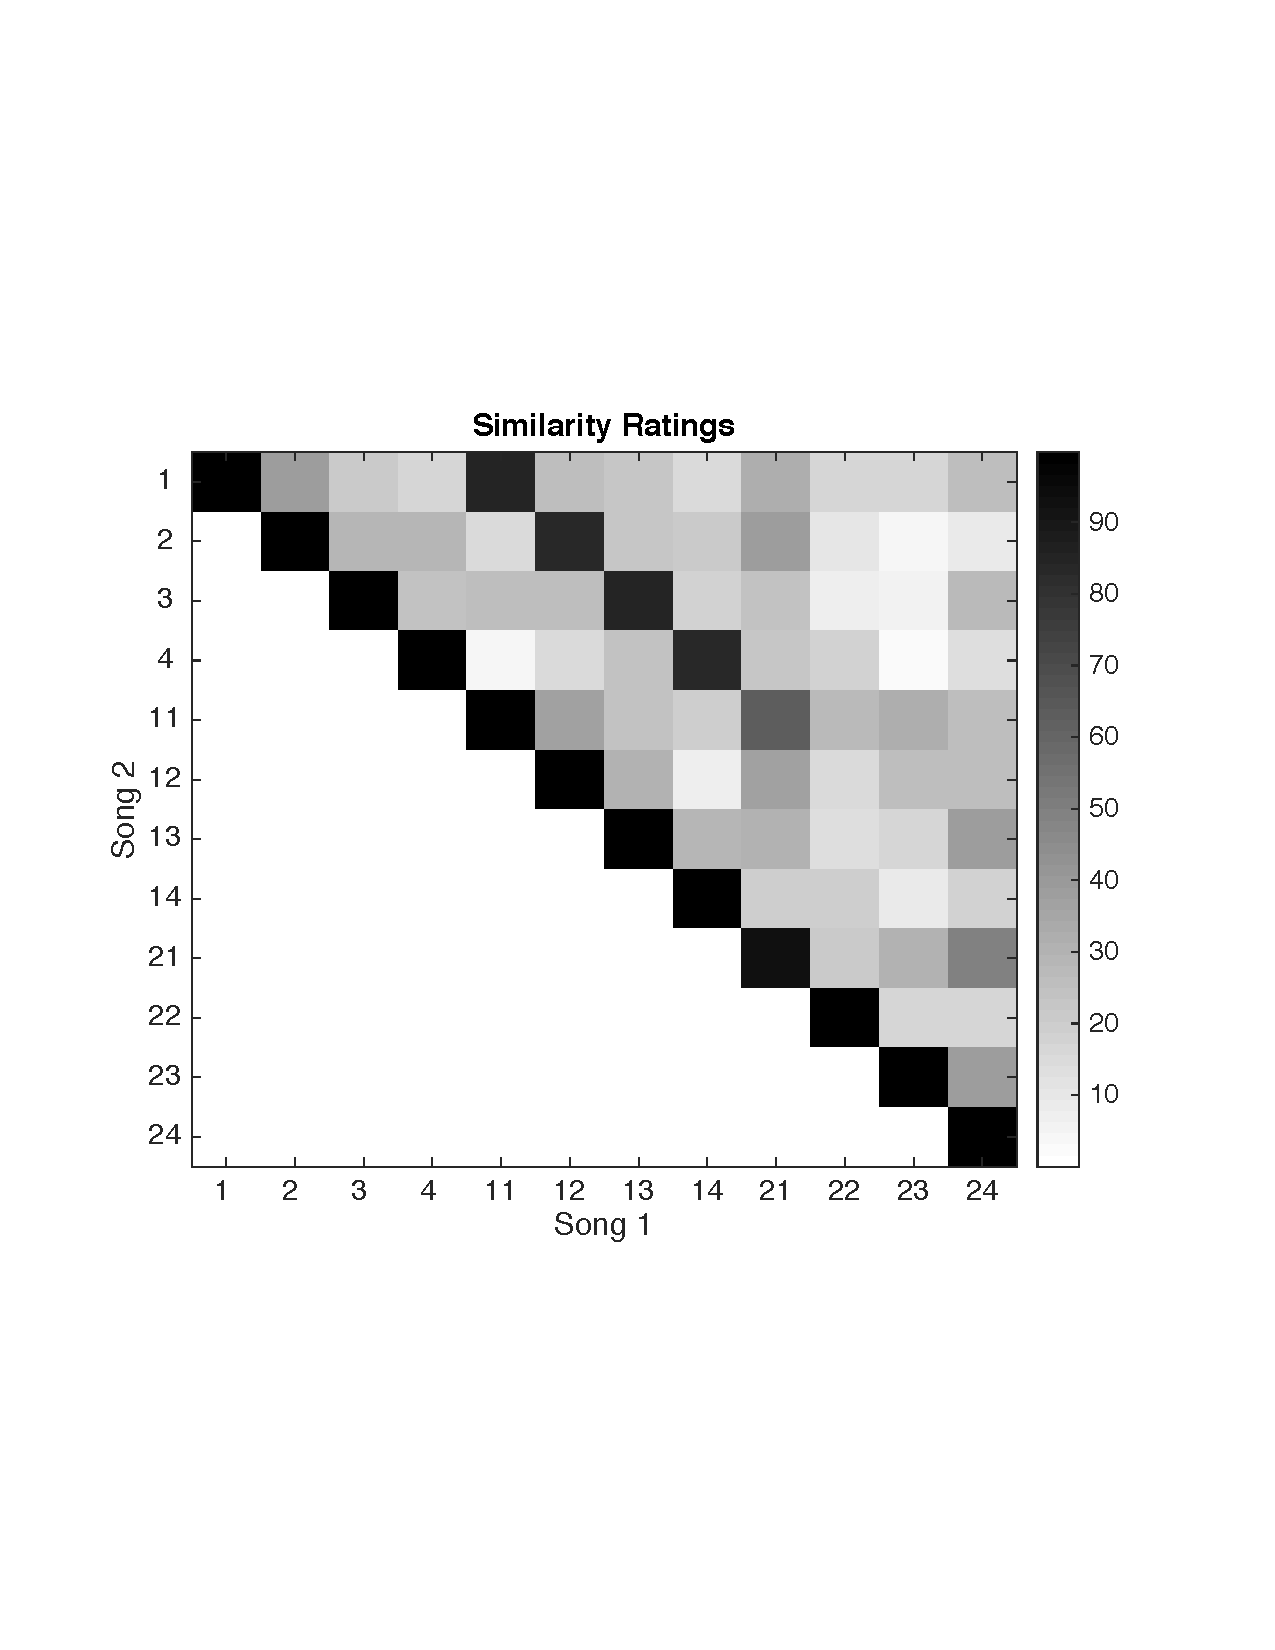
\includegraphics[width=\textwidth,keepaspectratio=true]{Figures/Similarity}
    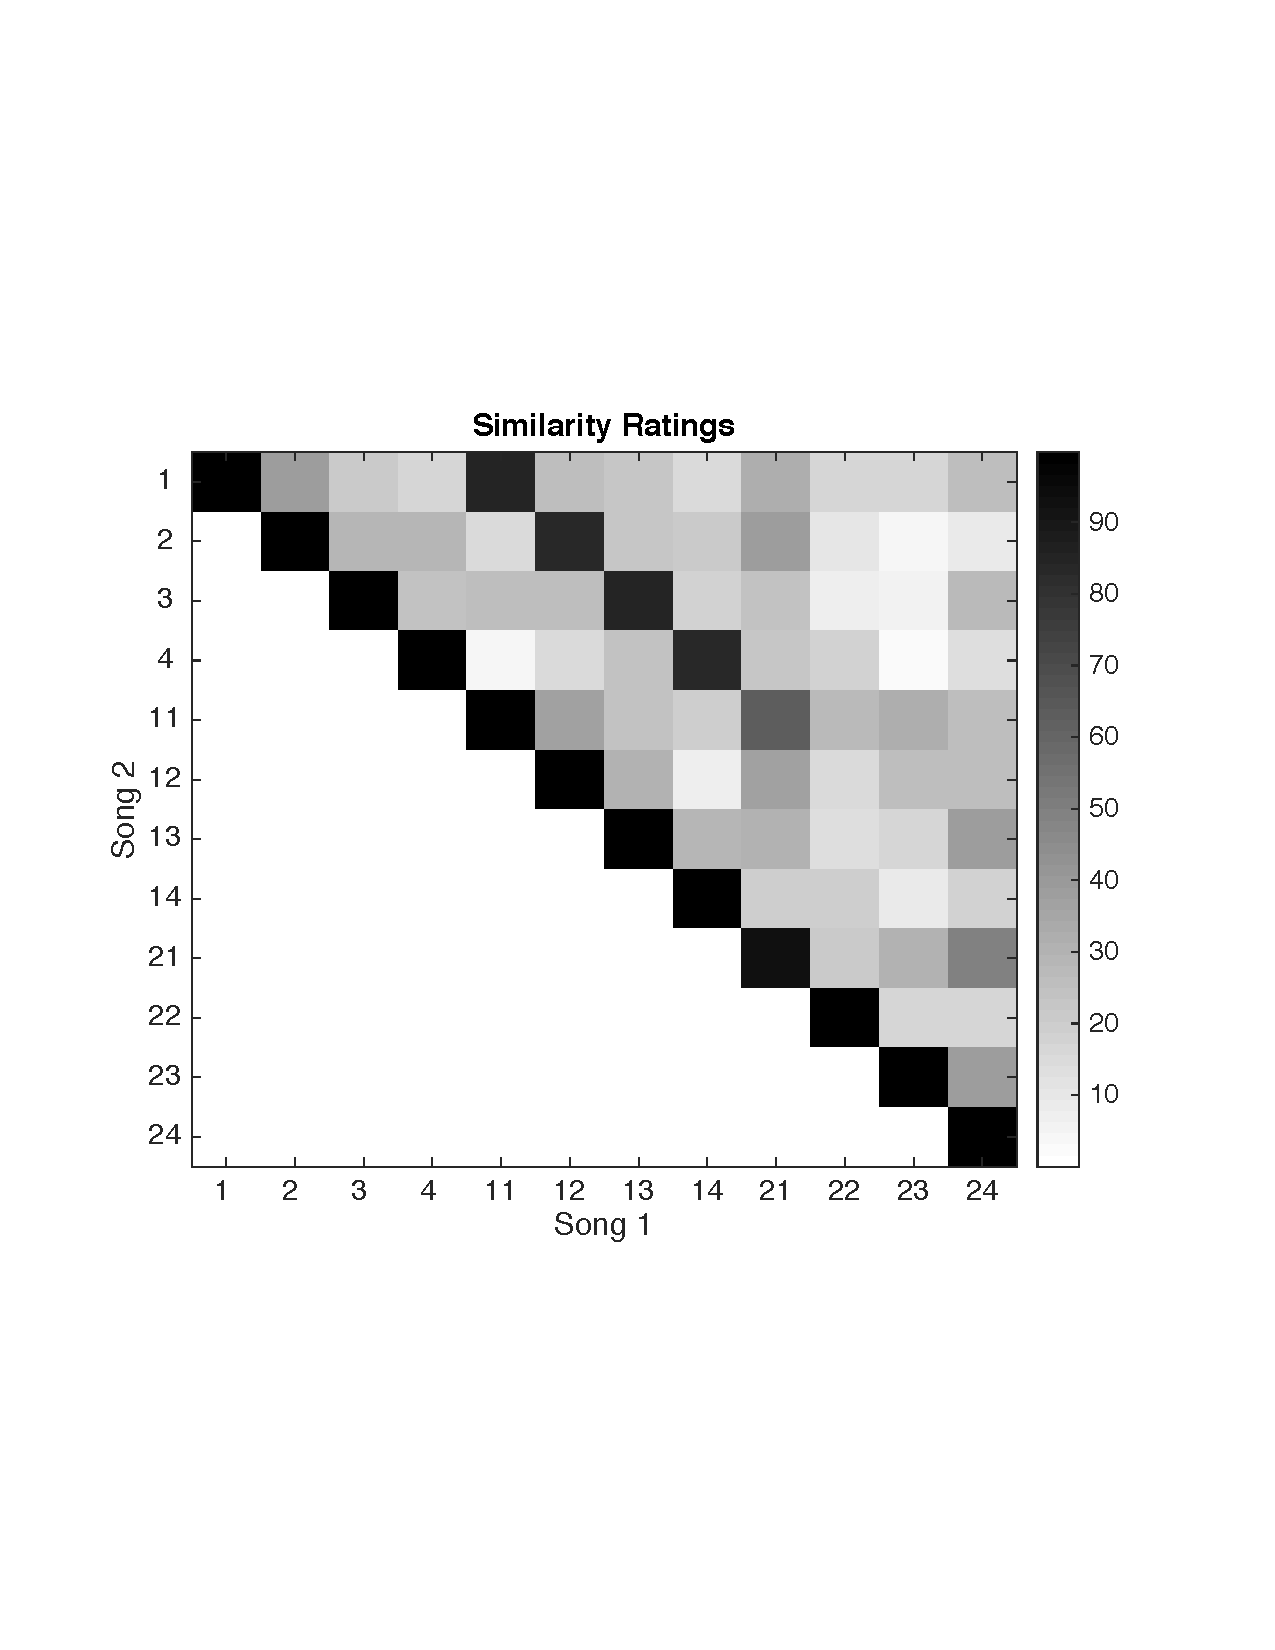
\includegraphics[scale=0.6]{Figures/Similarity}
%   \\\vspace{-0.8em}
    \caption{Similarity ratings (from 0-100) of binary comparisons of all stimuli.}
    \label{fig:Similarity}
  \end{center}
%  \vspace{-1em}
\end{figure}

\chapter{Discussion}
%\addcontentsline{toc}{chapter}{6. Discussion}
The goal of these experiments was to investigate whether the perception and imagination of short musical pieces could be classified using EEG.  
The ability to classify musical pieces from imagination could lead to the development of a \ac{BCI} that would allow patients with motor deficits to communicate through music imagination.
Ideally, patients would be able to imagine a piece of music to convey a certain thought (i.e. imagining ``Jingle Bells'' to indicate hunger).
Schaefer \etal \citeyear{schaefer_name_2011} were able to classify \emph{perceived} music stimuli based on the unique time courses of principal components that occurred during music perception, but we were unable to achieve the same result. 
The most likely reason is the number of stimuli presented to participants, as we presented far fewer trials per stimulus (5 vs 145). 
The small number of trials is also likely responsible for our inability to classify imagination using either the PCA technique or machine learning. 

The rationale for including so few trials per stimulus stemmed from the end-goal of building a music-based \ac{BCI}. 
A \ac{BCI} must operate with as little training as possible when used with patients.
The patients that require such interfaces to communicate may have difficulty directing attention, and focusing on a single task for a long time can be exhausting. 
A system that requires minimal training cuts down on patient fatigue during the training stage, ensuring that patients have enough energy to use the system for communication. 
Ideally, our \ac{BCI} would be trained on brain data collected during the \emph{perception} of music and tested on brain data collected during \emph{imagination} of music. 
By training on perception data we hoped to keep patient fatigue to a minimum. 
However, our results indicated that this is currently not a viable option with the existing data.  

Using machine learning techniques, we were able to train our system and classify the perception of music stimuli from the recorded EEG signal at a 29.6\% accuracy rate (chance = 17.59\%).
When investigating the pairs of stimuli that were most easily classified, there was no relationship to the energy attribute (calculated using EchoNest) of each musical piece (i.e., pieces with the most different energy levels were not more easily classifed). 
However, our neural network failed when applied to data collected during imagination of music.
The confusion matrix produced by the network (\autoref{fig:model_W_confusion_cond2}) is similar to what one would expect when trying to classify noise.
This result indicates that the system was not systematically misclassifying stimuli.

There are multiple reasons that could explain why we were unable to classify music imagination.
During perception, the timing of the music is consistent across trials (e.g. the second beat of the song always occurs at a consistent time point) because the timing is driven by the stimulus. 
During imagination, this timing may fluctuate across trials and across participants, because after the end of the tempo cue there is no external stimulus.
A single participant may imagine music at a different rate on different trials, and some participants may have a tendency to speed up or slow down throughout their imagining. 
Another inconsistency that may occur across participants, and across trials, is the focus of the imagination. 
It is possible that different participants focus on different aspects of the music while imagining.
Participants may choose to imagine the melody, the lyrics, or the instrumentation, and their focus may shift across trials.
There are also differences in `how' participants imagine music. 
After the experiment was completed, we asked participants what technique they used to imagine the music.
There was a 50-50 split between participants imagining themselves producing the music (i.e. singing the music) and participants ``hearing the music in their head''. 
Some participants also reported imagining vivid scenes, either from existing movies or completely novel scenes, to illustrate their music imagination.
This wide array of differences is likely the cause of our low imagination classification rates. 

The secondary goal of these experiments was to determine what neural processes drive the classification of music perception and imagination.
Although it is tempting to interpret the results of a neural network, it is difficult to determine why a trained neural network makes a particular decision \cite{towell_1992_interpretation}.
One way of understanding a neural network's decisions is by investigating the layers of the network separately and relating the weights within these layers to the input and the output. 
However, understanding the structure of a neural network may not necessarily inform us about what the brain is doing to perform the same task. 
%There are a few things to keep in mind about neural network solutions. 
First, the network's solution may not be unique and may simply be one of many possible solutions. 
Although the network is constrained to minimize misclassification error, the solution reached by the network could be a local minimum -- the best solution for this particular combination of parameters.
The network tries out different combinations of parameters until it finds a solution that it decides best minimizes misclassification error. 
However, with further tweaking of the network, and a different combination of parameters, there may be a solution that minimizes the misclassification error further.
It is impossible to know whether the network's solution is the global minimum -- the solution with the lowest possible misclassification error.
%It may be possible to uncover the global minimum of the problem, but there is no way to be sure that the global minimum has been reached.
Second, interpretation is difficult because a solution is reached based on parameters set by the researcher. 
It is not possible to untangle whether aspects of the solution are necessary for solving the problem or if they are influenced by the chosen network architecture. 
Lastly, artificial neural networks, like the one used in this experiment, are \emph{artificial}, and only superficially resemble the way a biological system processes information. 
It is not possible to know whether the way an artificial network solves a biological problem is the same way a biological system would solve it. 

However, to investigate whether we could glean any brain-related information from our neural network (\autoref{fig:model_W}), we focused on whether the spatial or temporal filters could be related to any biological or musical characteristics.
The spatial filter in layer 1 indicated which electrodes carried the \ac{EEG} data important for classification. 
However, because of the spatially imprecise nature of \ac{EEG}, we are unable to comment on where the data from these electrodes is produced.
\ac{EEG} collects electrical signals at the scalp that are produced by the brain.
By the time the electrical information reaches the electrodes, it has travelled through layers of tissue and the skull and is diffuse.
Trying to reconstruct the sources of the electrical signal in three dimensional space presents a reverse inference problem with countless solutions.
Because there is more than one way to identify sources within the brain that could produce the electrical signal patterns recorded at the scalp, it is very difficult to pinpoint where the signals collected by each electrode originated.

One approach to breaking an EEG signal down into constituent parts is to use \ac{PCA}.
The auditory research literature is in consensus on what principal components of auditory processing look like.
However, the spatial filter in layer 1 does not match what is seen in a \ac{PCA} of auditory \ac{EEG}.
Generally auditory component peaks are located in the fronto-central region of the topographic spatial map. 
The layer 1 filter does not have any similarities to the biologically produced components and has lateral peaks. 
Because we could not relate the layer 1 filter to any biological information, and we had no way to interpret what type of signals are picked up by the electrodes the model has labeled as important for classification, we decided to force the net to use biologically produced information to see whether the model's classification abilities change. 
We exchanged the neural net's first layer with the principal components calculated in \autoref{fig:components}C. 
This resulted in a decrease in classification accuracy. The results from the neural net using biologically produced spatial maps can be seen in Appendix \ref{appendix:PCAInvestigation}.

The second and third layers of the neural net produced temporal filters and compressed representations of the data that highlight time periods in the stimuli that are important for classification. 
Upon closer investigation there were no auditory characteristics that stood out as being unique to each of the important time periods.
These time periods did not relate to salient auditory events, important points in the musical structure of the piece, or any obvious aspect of the lyrics, such as word repetition. 
To determine whether the patterns in the filters were driven by a cognitive process such as recognition of the music we conducted a behavioural experiment.
The results showed that the highlighted time periods do not coincide with the moment participants recognized the piece of music. 
\autoref{fig:RecognitionTime} shows that participants consistently recognize the pieces of music well before the important time periods occur in the temporal filters. 
Based on these results we know what is \emph{not} responsible for highlighting these moments in the classifier: the importance of these moments is not due to auditory characteristics of the stimuli or a moment of recognition.
At this time we are unable to say what is causing these time periods to be flagged as important for stimulus classification. 

Although we were able to classify music perception (accuracy = 29.6\%), we were not able to classify music imagination (accuracy = 7.4\%).
Future experiments should aim to disentangle what information is driving the classifier during perception and to enhance this during imagination.
To do this we may need to use simpler stimuli.
Rhythm stimuli are simpler than music stimuli because they do not include melody, lyric, or instrumentation information. 
If we are able to classify the imagination of rhythmic stimuli more accurately than the imagination of music then we may be able to say that it is the rhythmic component of music driving the classification in this experiment.
Then, one at a time, we can add in other aspects of music like tone and lyrics to determine what effect they have on classification accuracy until we reach the optimum combination of musical characteristics.
Previous research has shown that it is possible to classify the perception of rhythms \cite{stober2014audiomostly}, so capitalizing on rhythm's auditory simplicity may be an effective way to learn what characteristics are necessary to drive a music-based \ac{BCI}.
Finally, it will also be important during future experiments to continue to cue participants to the tempo during imagination using a metronome.
This will ensure that all participants imagine at the same rate and are consistent across multiple trials.
\end{spacing}

%% This adds a line for the Bibliography in the Table of Contents. (called Bibliography rather than automatic "References")
%\addcontentsline{toc}{chapter}{Bibliography}
%% ***   Set the bibliography style.   ***
\bibliographystyle{apacite} % (change according to your preference)
%%% ***   Set the bibliography file.   ***
\bibliography{Bibliography}{}
%Appendices.
\begin{appendices}
\chapter{Ethics Approval Form}\label{appendix:ethics}
\myappendices{Appendix \ref{appendix:ethics} {Ethics Approval Form}}

The Ethics Approval Form can be found on the following page.
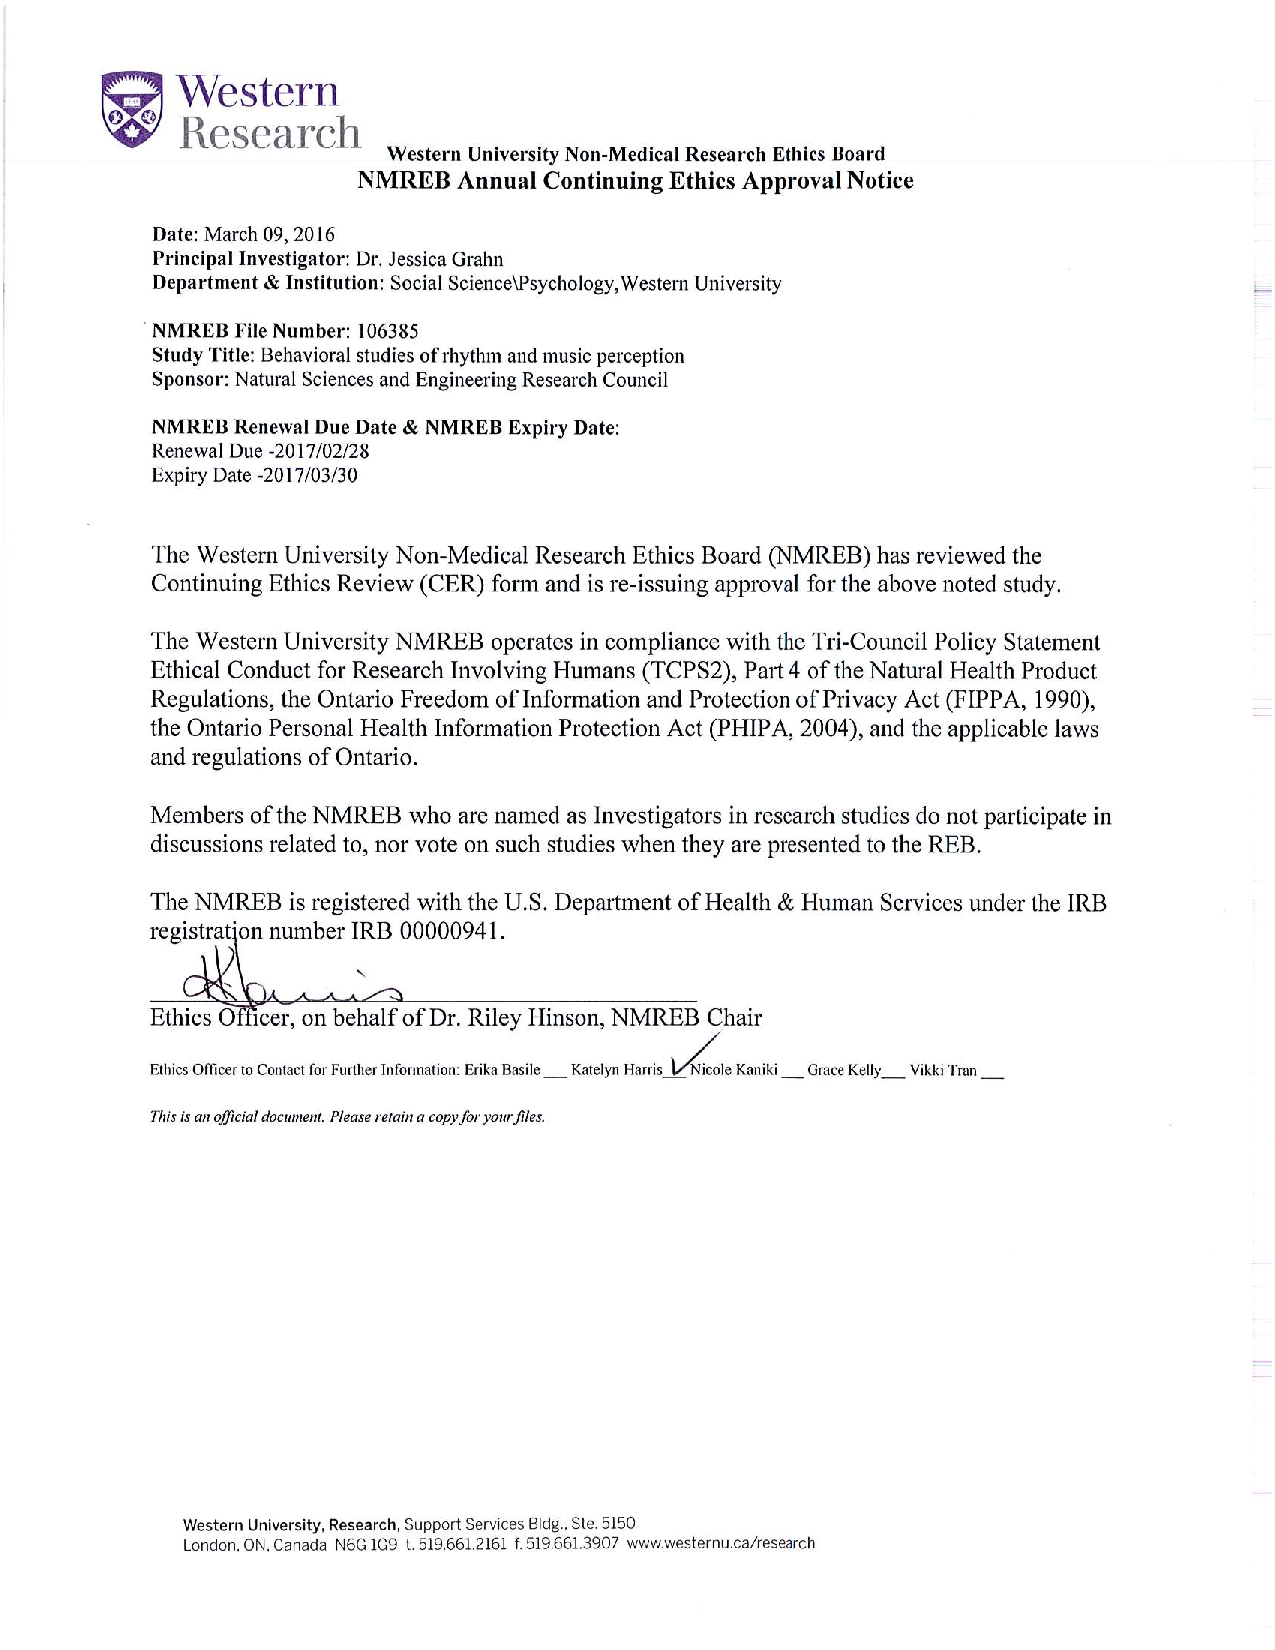
\includepdf{Figures/EthicsApproval.pdf}
\chapter{Questionnaire}\label{appendix:questionnaire}
\myappendices{Appendix \ref{appendix:questionnaire} {Questionnaire}}

The questionnaire used during both the EEG and the behavioural experiment can be found on the following pages.
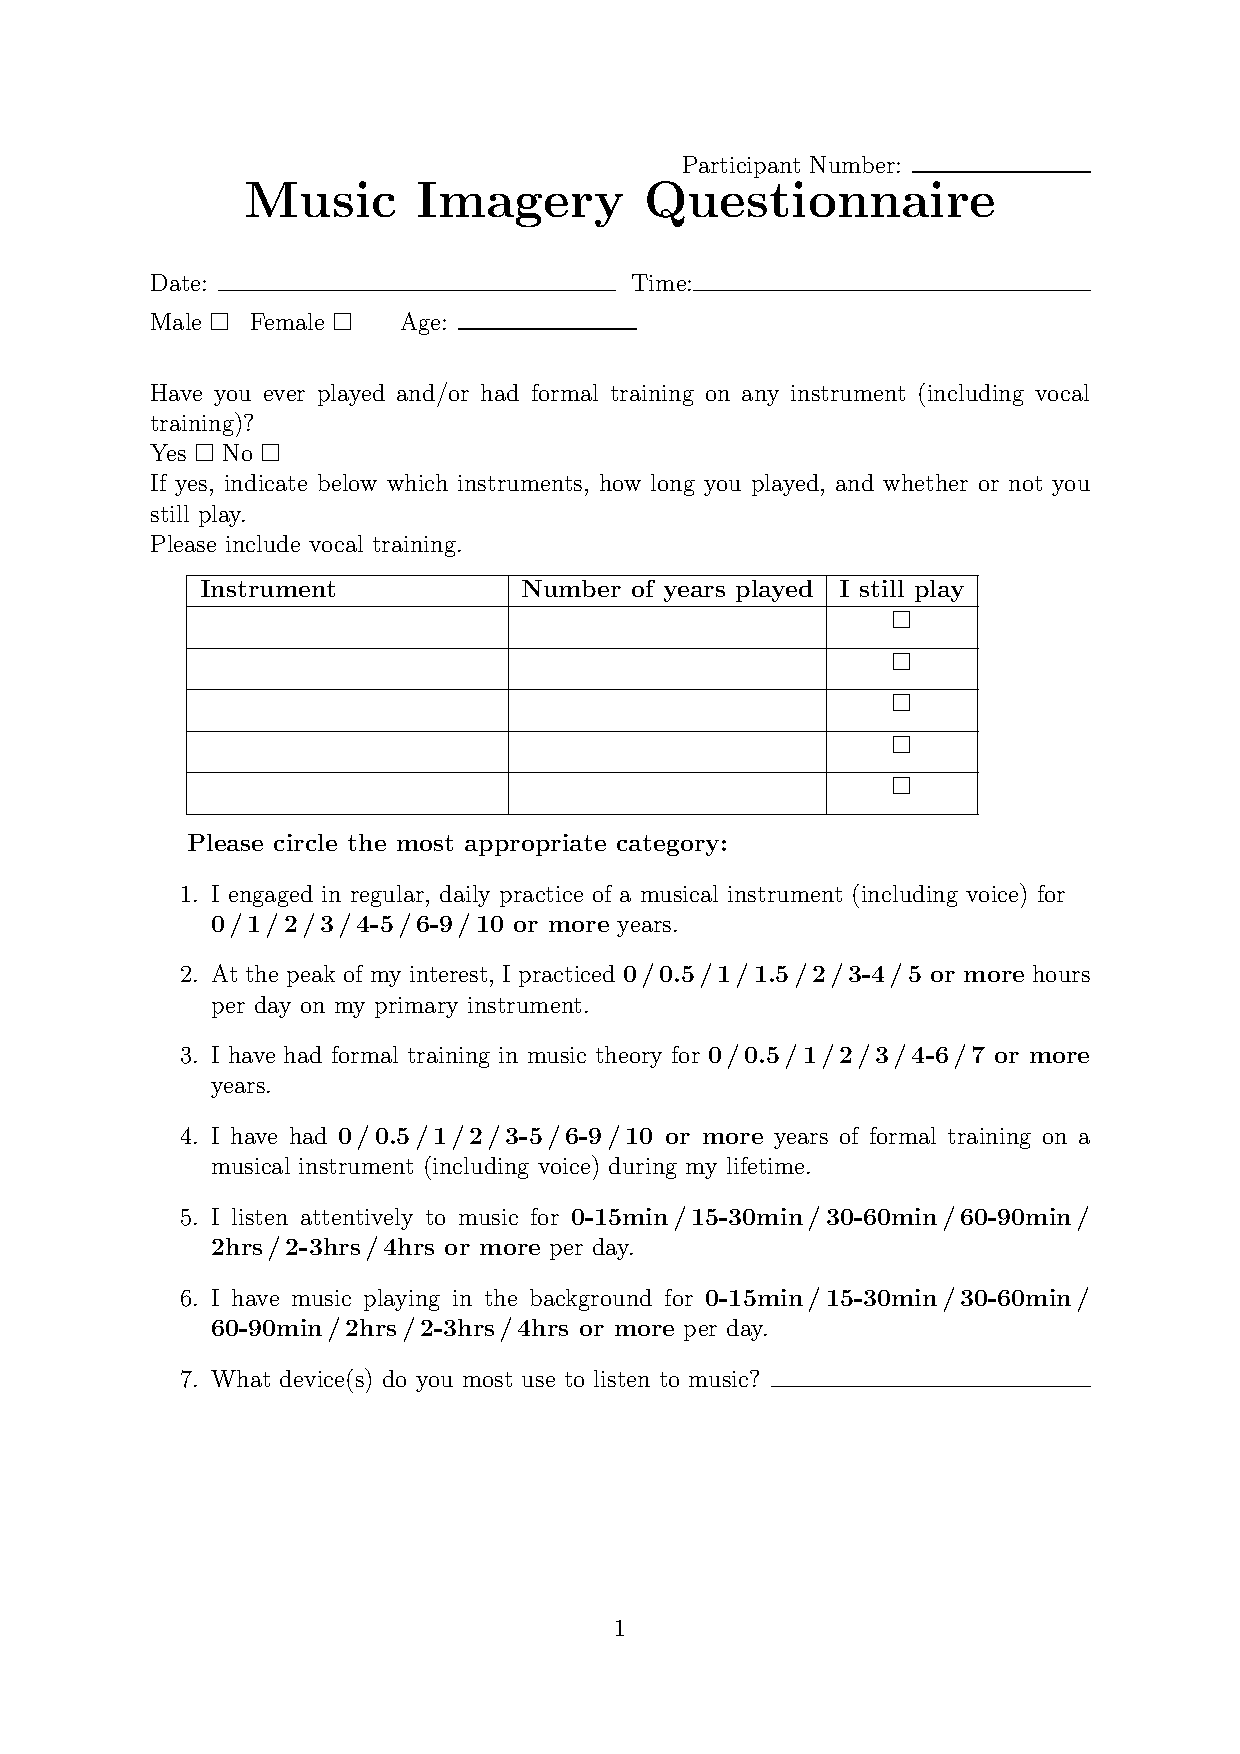
\includepdf[pages={1,2}]{Figures/questionnaire.pdf}

\chapter{PCA Filters in Layer 1}
\begin{figure}[h] 
  \begin{center}
   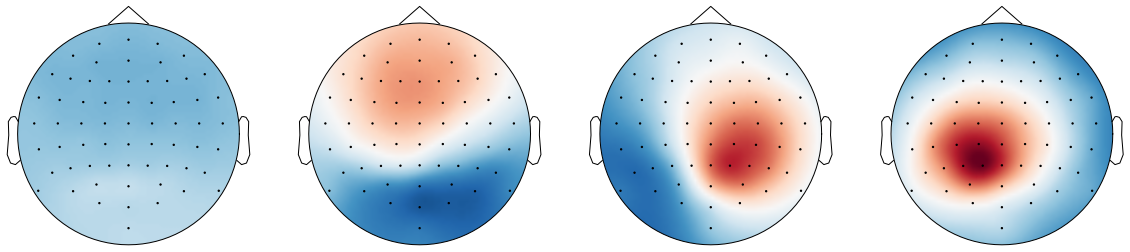
\includegraphics[width=.5\textwidth,keepaspectratio=true]{Figures/PCA_SVM}
   \\\vspace{-0.8em}
    \caption{PCA done on training trials}
    \label{fig:PCA_SVM}
  \end{center}
  \vspace{-1em}
\end{figure}

\begin{figure}[h] 
  \begin{center}
%  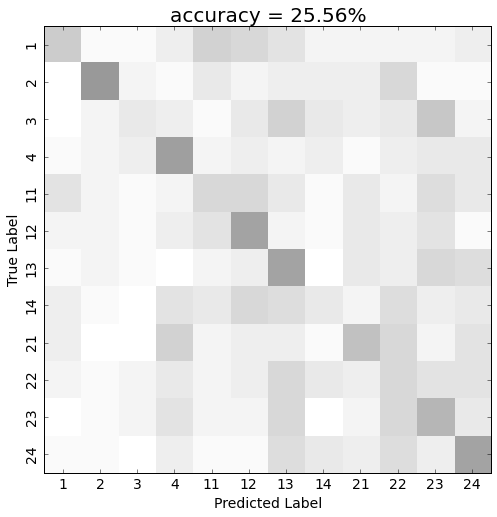
\includegraphics[width=.5\textwidth,keepaspectratio=true]{Figures/PC0_confusion}
    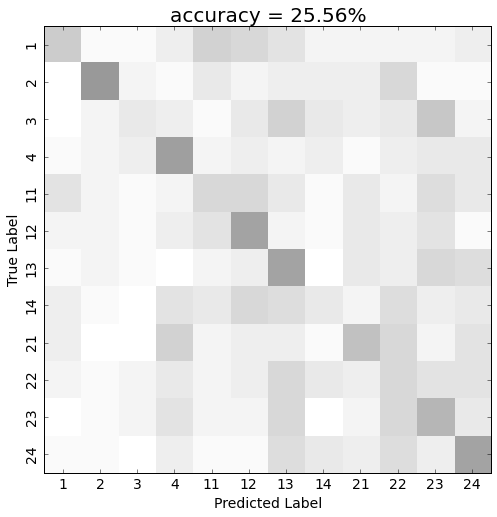
\includegraphics[scale=0.5]{Figures/PC0_confusion}
   \\\vspace{-0.8em}
    \caption{Replacing layer 1 with PC 0}
    \label{fig:PC0_confusion}
  \end{center}
  \vspace{-1em}
\end{figure}

\begin{figure}[h] 
  \begin{center}
%    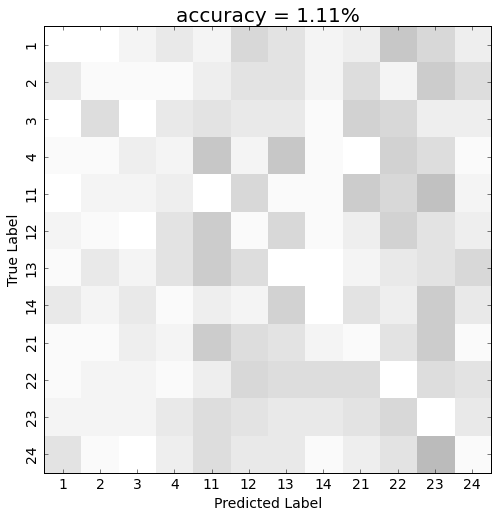
\includegraphics[width=.5\textwidth,keepaspectratio=true]{Figures/PC1_confusion}
    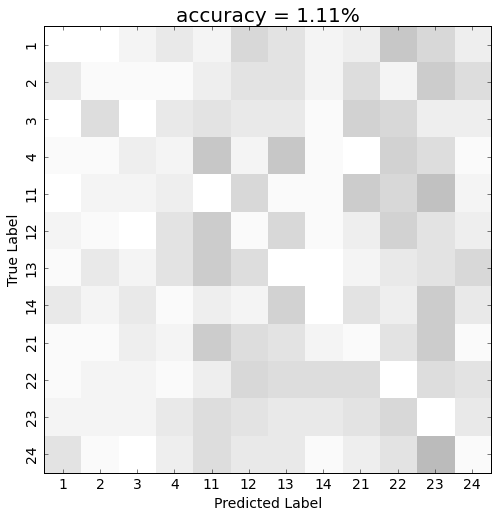
\includegraphics[scale=0.5]{Figures/PC1_confusion}
   \\\vspace{-0.8em}
    \caption{Replacing layer 1 with PC 1}
    \label{fig:PC1_confusion}
  \end{center}
  \vspace{-1em}
\end{figure}

\begin{figure}[h] 
  \begin{center}
%    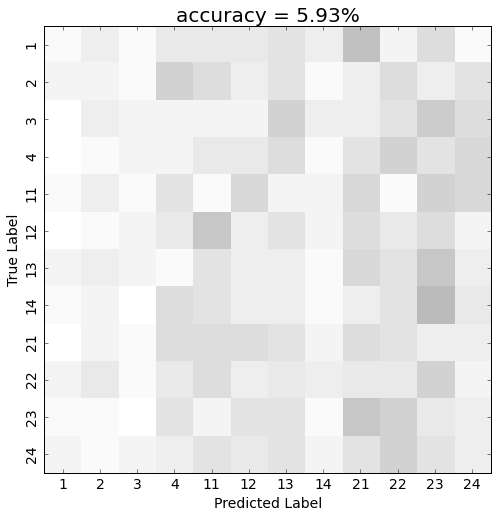
\includegraphics[width=.5\textwidth,keepaspectratio=true]{Figures/PC2_confusion}
    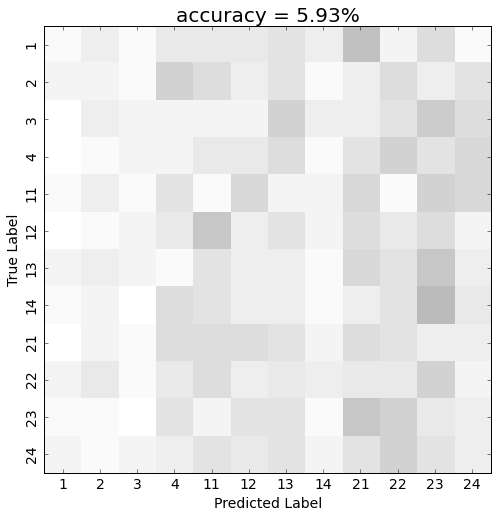
\includegraphics[scale=0.5]{Figures/PC2_confusion}
   \\\vspace{-0.8em}
    \caption{Replacing layer 1 with PC 2}
    \label{fig:PC2_confusion}
  \end{center}
  \vspace{-1em}
\end{figure}

\begin{figure}[h] 
  \begin{center}
%    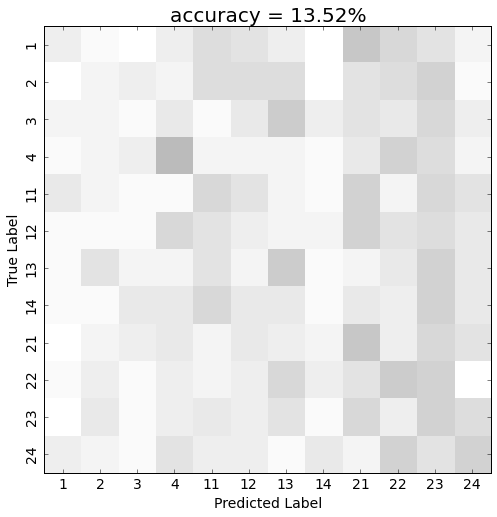
\includegraphics[width=.5\textwidth,keepaspectratio=true]{Figures/PC3_confusion}
    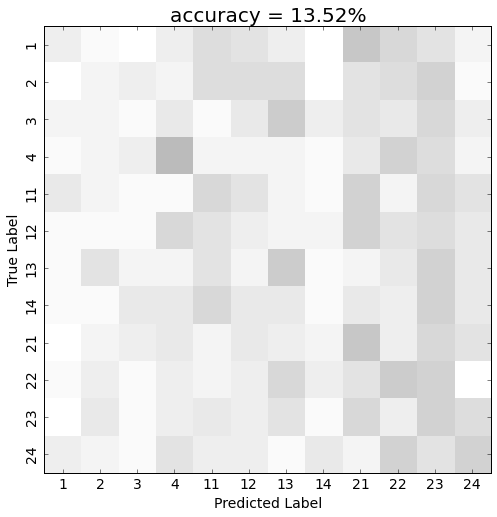
\includegraphics[scale=0.5]{Figures/PC3_confusion}
   \\\vspace{-0.8em}
    \caption{Replacing layer 1 with PC 3}
    \label{fig:PC3_confusion}
  \end{center}
  \vspace{-1em}
\end{figure}
\end{appendices}
%CV only relevant stuff... not full CV.
\addcontentsline{toc}{chapter}{Curriculum Vitae}
%\chapter*{Curriculum Vitae}
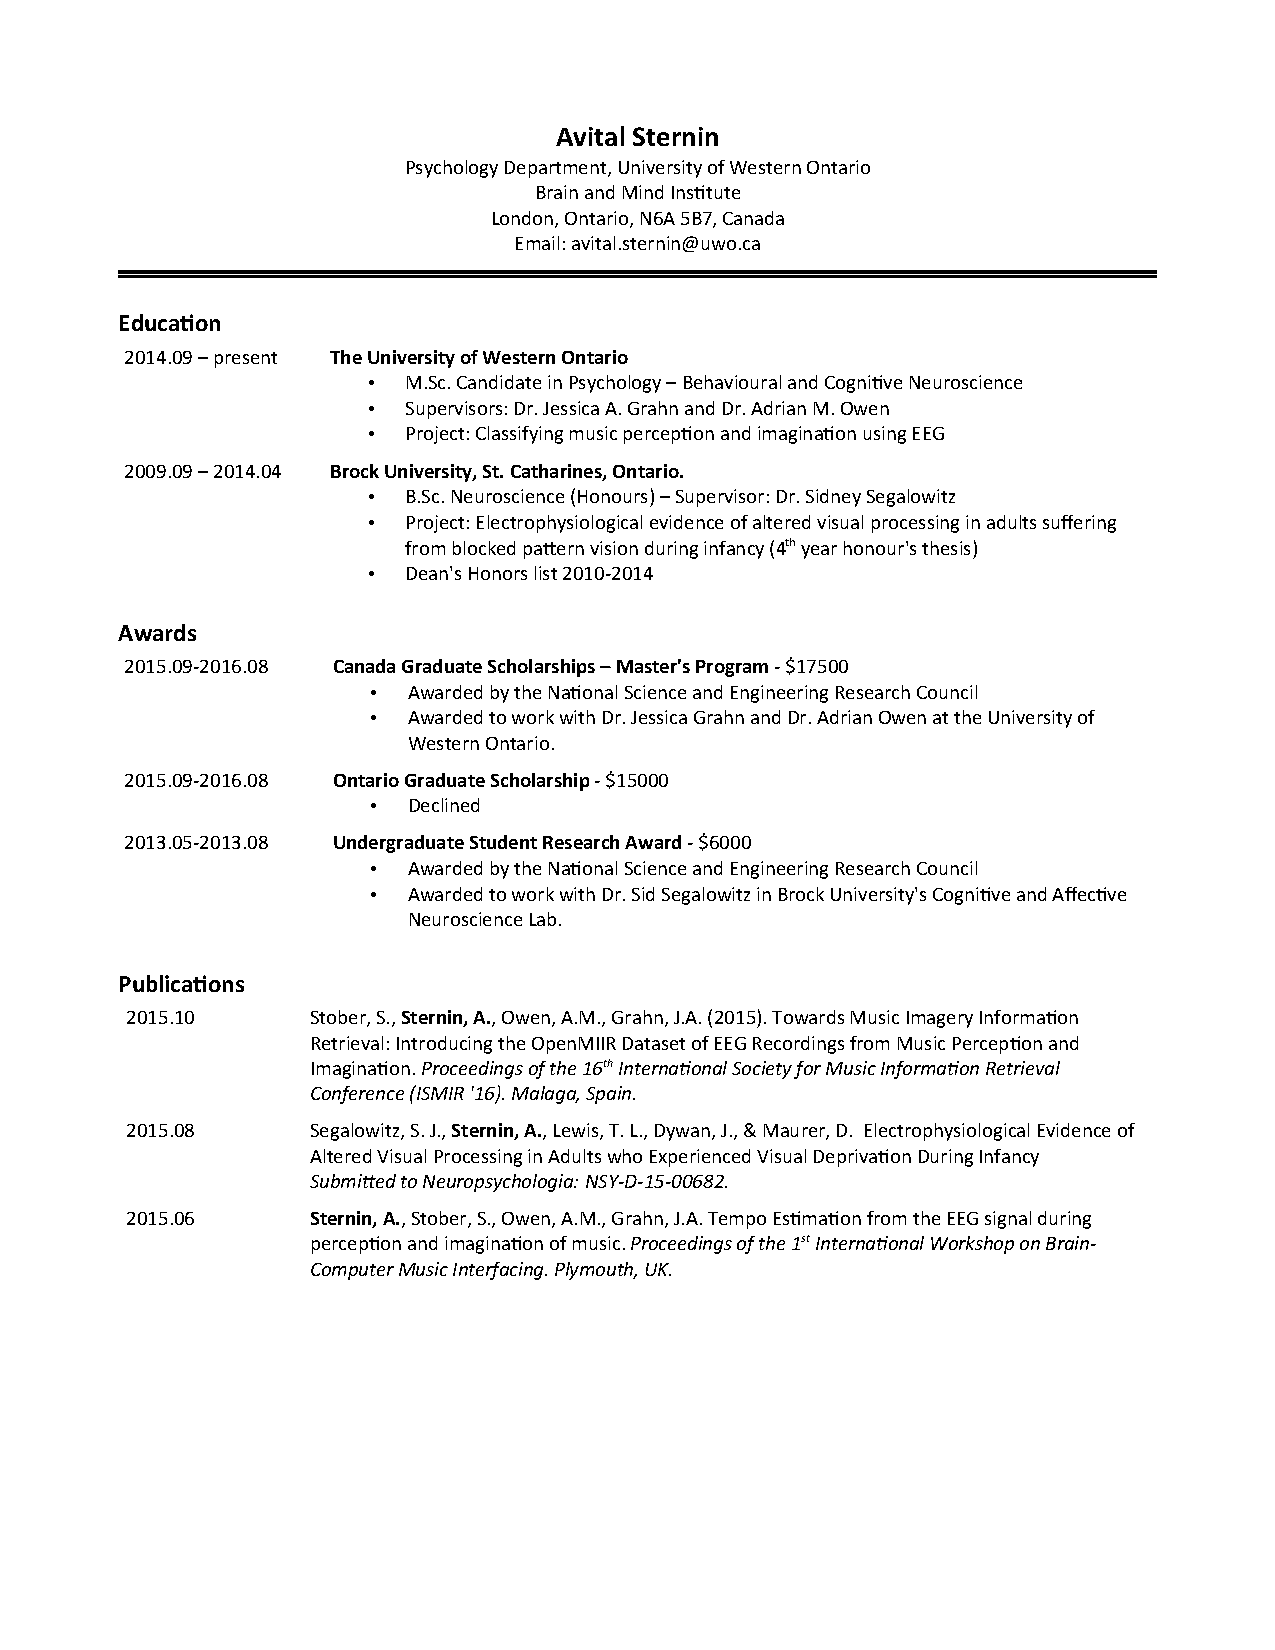
\includepdf[pages={1,2}]{Chapters/CV-MScThesis.pdf}
\end{document}

